%; whizzy paragraph
%; whizzy-paragraph "^\\\\dancersection"
% -initex iniptex -latex platex -format platex -bibtex jbibtex -fmt fmt
% 以上 whizzytex を使用する場合の設定。

%     Tokyo Debian Meeting resources
%     Kansai Debian Meeting resources
%     Copyright (C) 2012 Junichi Uekawa
%     Copyright (C) 2012 Nobuhiro Iwamatsu
%     Copyright (C) 2012 Koichi Akabe

%     This program is free software; you can redistribute it and/or modify
%     it under the terms of the GNU General Public License as published by
%     the Free Software Foundation; either version 2 of the License, or
%     (at your option) any later version.

%     This program is distributed in the hope that it will be useful,
%     but WITHOUT ANY WARRANTY; without even the implied warranty of
%     MERCHANTABILITY or FITNESS FOR A PARTICULAR PURPOSE.  See the
%     GNU General Public License for more details.

%     You should have received a copy of the GNU General Public License
%     along with this program; if not, write to the Free Software
%     Foundation, Inc., 51 Franklin St, Fifth Floor, Boston, MA  02110-1301 USA

%  preview (shell-command (concat "evince " (replace-regexp-in-string "tex$" "pdf"(buffer-file-name)) "&"))
% 画像ファイルを処理するためにはebbを利用してboundingboxを作成。
%(shell-command "cd image2012-natsu; ebb *.png")

% progress memo:
% 2014/12-2015/05がマージ対象、関西は2014/12-2015/05
% イベント等でない場合は理由を書くこと。
% 必要な変更点は FIXME で記録しています。

%%ここからヘッダ開始。

\documentclass[mingoth,a4paper]{jsarticle}
\usepackage{monthlyreport}
\usepackage{supertabular}
\usepackage{subfigure}
\renewcommand*\thesubfigure{}

\usepackage{comment}

% ルビ for 201312tokyo
\def\ruby#1#2{%
\leavevmode
\setbox0=\hbox{#1}\setbox1=\hbox{\tiny#2}%
\ifdim\wd0>\wd1 \dimen0=\wd0 \else \dimen0=\wd1 \fi
\hbox{\kanjiskip=\fill
\vbox{\hbox to \dimen0{\tiny \hfil#2\hfil}%
\nointerlineskip
\hbox to \dimen0{\hfil#1\hfil}}}}

% section の代わりの環境 -- 改訂する。
\renewcommand{\dancersection}[2]{%
\newpage
あんどきゅめんてっど でびあん 2015年夏号
%
% top line
\vspace{0.1mm}\\
{\color{dancerdarkblue}\rule{\hsize}{2mm}}

%
% middle text
%
\begin{minipage}[t]{0.6\hsize}
\color{dancerdarkblue}
\vspace{1cm}
\section{#1}
\hfill{}#2\\
\end{minipage}
\begin{minipage}[t]{0.4\hsize}
\vspace{-2cm}
\hfill{}
\includegraphics[height=8cm]{image200502/openlogo-nd.eps}\\
\vspace{-5cm}
\end{minipage}
%
% bottom line
{\color{dancerlightblue}\rule{0.66\hsize}{2mm}}
%
\vspace{2cm}
}
% end of dancersection.

\begin{document}

\begin{titlepage}
\thispagestyle{empty}

\hspace*{-2.5cm}
\includegraphics{image2012-natsu/gudeb.eps}\\
\vspace*{0.1cm}

\vspace*{2cm}
\rotatebox{10}{\fontsize{32}{32} {\gt 東京エリア/関西Debian勉強会}}

\vspace*{-1.5cm}
\hspace*{11cm}
\includegraphics[height=6cm]{image200502/openlogo-nd.eps}\\
\vspace*{0.1cm}
\hfill あんどきゅめんてっど でびあん 2015年夏号 2015年8月16日 初版発行
\end{titlepage}

\newpage
\thispagestyle{empty}\mbox{}
\newpage

\setcounter{page}{1}
\begin{minipage}[]{0.2\hsize}
 \definecolor{titleback}{gray}{0.9}
 \colorbox{dancerlightblue}{\rotatebox{90}{\fontsize{80}{80}
{\gt \color{dancerdarkblue}デビアン勉強会} }}
\end{minipage}
\begin{minipage}[]{0.8\hsize}
\hrule
\vspace{1mm}
\hrule
\setcounter{tocdepth}{1}
{\small
\begin{multicols}{2}
  \tableofcontents
\end{multicols}
} %FIXME: does not fit in one column! しかし二段にするとあまり美しくない? 真ん中のあたりで章番号とページ数の番号が近くにあるのがバランス良くない気がする
\vspace{1mm}
\hrule
\vspace{3cm}

\end{minipage}

% FIXME: 本文を追加すること。
%-------------------------------------------------------------------------------
\dancersection{Introduction}{上川 純一, 山下 尊也}
%-------------------------------------------------------------------------------

\subsection{東京エリアDebian勉強会}

 Debian勉強会へようこそ。これからDebianの世界にあしを踏み入れると
 いう方も、すでにどっぷりとつかっているという方も、月に一回Debianについ
 て語りませんか?

 Debian勉強会の目的は下記です。

\begin{itemize}
 \item \underline{Debian Developer} (開発者)の育成。
 \item 日本語での「\underline{開発に関する情報}」を整理してまとめ、アップデートする。
 \item \underline{場}の提供。
 \begin{itemize}
  \item 普段ばらばらな場所にいる人々が face-to-face で出会える場を提供
	する。
  \item Debian のためになることを語る場を提供する。
  \item Debianについて語る場を提供する。
 \end{itemize}
\end{itemize}

 Debianの勉強会ということで究極的には参加者全員がDebian Packageをがりがり
 と作るスーパーハッカーになった姿を妄想しています。情報の共有・活用を通し
 て Debianの今後の能動的な展開への土台として、「場」としての空間を提供す
 るのが目的です。

\subsection{関西 Debian 勉強会}

 関西 Debian 勉強会はDebian GNU/Linux のさまざ
 まなトピック(新しいパッケージ、Debian 特有の機能の仕組、Debian 界隈で起
 こった出来事、などなど)について話し合う会です。

 目的として次の三つを考えています。
 \begin{itemize}
  \item メーリングリストや掲示板ではなく、直接顔を合わせる事での情報交換の促進
  \item 定期的に集まれる場所
  \item 資料の作成
 \end{itemize}

 それでは、楽しい一時をお楽しみ下さい。

%-------------------------------------------------------------------------------
% end of header
%-------------------------------------------------------------------------------

\clearpage
\newpage
%201504kansai
\dancersection{Wheezy から Jessie まで}{かわだてつたろう}

Debian 8 Jessie がリリースされました。

今回もリリースまでに色々とありましたので、WheezyリリースからJessieリリースまでを
関西Debian勉強で何度かご紹介してきたDebian Projectの近況から振り返ってみましょう。

\subsection{Wheezyリリース}

Debian 7 Wheezyは2012年6月30日にフリーズされ
\footnote{\url{https://lists.debian.org/debian-devel-announce/2012/06/msg00009.html}}、
一年近くのフリーズ期間を経て、2013年5月4日にリリースされました。
\footnote{\url{http://www.debian.org/News/2013/20130504}}

ここからJessieの開発が始まります。


\subsection{2013年}

5月6日、Jessieの開発が宣言
\begin{quote}
  「Wheezy is out! Jessie is created and receives updates!」
  \footnote{\url{http://lists.debian.org/debian-devel-announce/2013/05/msg00004.html}}
\end{quote}

8月11日〜18日、DebConf 13がスイスのヴォーマルキュで開催
\footnote{\url{http://debconf13.debconf.org/}}

8月25日、リリースチームより開発サイクルの提案
\begin{quote}
  「Bits from the Release」
  \footnote{\url{http://lists.debian.org/debian-devel-announce/2013/08/msg00006.html}}
\end{quote}

\begin{screen}
  \begin{itemize}
  \item Changing testing migration (NEW-TEST)
  \item Key-packages and automated removals (AUTO-RM)
  \item Automating Architecture (re-)Qualification (ARCH)
  \item Roll call for porters (ROLL-CALL)
  \end{itemize}
\end{screen}

9月11日、リリースチームからリリースゴールの呼び掛け
\begin{quote}
  「Call for Jessie Release Goals」
  \footnote{\url{http://lists.debian.org/debian-devel-announce/2013/09/msg00001.html}}
\end{quote}

\begin{screen}
  \begin{itemize}
  \item Native systemd support in every package with sysv scripts
  \item Hardening of ELF binaries (carry over from Wheezy)
  \item debian/rules to honor CC/CXX flags
  \item clang as secondary compiler
  \item piuparts clean archive
  \item Cross Toolchains in the archive
  \item Make the base system cross-buildable
  \item SELinux
  \item UTF-8
  \end{itemize}
\end{screen}

10月13日、フリーズ日が2014年11月5日 23時59分(UTC)になるとアナウンス
\begin{quote}
  「Bits from the Release Team (Jessie freeze info)」
  \footnote{\url{http://lists.debian.org/debian-devel-announce/2013/10/msg00004.html}}
\end{quote}

11月28日、対象アーキテクチャからs360とia64が除外
\begin{quote}
  「Release sprint results - team changes, auto-rm and arch status」
  \footnote{\url{http://lists.debian.org/debian-devel-announce/2013/11/msg00007.html}}
\end{quote}


\subsubsection{systemd}

フリーズ日のアナウンスがされる前後に、
\begin{quote}
  「systemd effectively mandatory now due to GNOME」
  \footnote{\url{http://lists.debian.org/debian-devel/2013/10/msg00444.html}}
\end{quote}
から始まって、
\begin{quote}
  「Proposal: switch default desktop to xfce」
  \footnote{\url{http://lists.debian.org/debian-devel/2013/10/msg00496.html}}
\end{quote}
に続き、
\begin{quote}
  「Proposal: switch init system to systemd or upstart」
  \footnote{\url{http://lists.debian.org/debian-devel/2013/10/msg00651.html}}
\end{quote}
へと、systemdの話題でdebian-devel@debian.orgを賑わせることとなりました。

systemdに関する話題はその後も続くことになります。


\subsection{2014年}

明けて2014年、2月11日にJessieからLinuxアーキテクチャのinit systemをsystemdとする
CTTEの決定がアナウンスされます。
\begin{quote}
  「[CTTE \#727708] Default init system for Debian」
  \footnote{\url{https://lists.debian.org/debian-devel-announce/2014/02/msg00005.html}}
\end{quote}

この決定に端を発してdebian-devel@debian.orgは荒れに荒れ、「Code of Conduct」
\footnote{\url{https://www.debian.org/vote/2014/vote_002}}
の採択へと繋がります。

その一方でJessieの開発は着々と進んでおり

3月19日、インストーラチームからDebian Installer Jessie Alpha1がリリース
\begin{quote}
  「Debian Installer Jessie Alpha1 release」
  \footnote{\url{https://www.debian.org/devel/debian-installer/News/2014/20140319}}
\end{quote}

4月26日、SPARCがリリースアーキテクチャから取り除かれる
\begin{quote}
  「SPARC removed from Jessie」
  \footnote{\url{https://lists.debian.org/debian-devel-announce/2014/04/msg00012.html}}
\end{quote}

5月1日、リリースチームからは6ヶ月を切ったフリーズまでのタイムテーブルが報告
\begin{quote}
  「Bits from the Release Team - Freeze, removals and archs」
  \footnote{\url{https://lists.debian.org/debian-devel-announce/2014/05/msg00000.html}}
\end{quote}

5月22日、Debian GNU/Hurdが80\%のパッケージをカバーしSysVinitが動作することなどの活動報告
\begin{quote}
  「Bits from the Debian GNU/Hurd porters」
  \footnote{\url{https://lists.debian.org/debian-devel-announce/2014/05/msg00006.html}}
\end{quote}

6月3日、MATE Packaging TeamよりMATE 1.8のDebian入りが報告
\begin{quote}
  「MATE 1.8 has now fully arrived in Debian」
  \footnote{\url{https://lists.debian.org/debian-devel/2014/06/msg00041.html}}
\end{quote}

6月18日、libcがeglibcからglibcに戻る
\begin{quote}
  「Accepted glibc 2.19-3experimental0 (source all)」
  \footnote{\url{https://packages.qa.debian.org/g/glibc/news/20140618T220008Z.html}}
\end{quote}

7月30日、Debian LinuxカーネルチームよりJessieのLinuxカーネルを3.16にすると報告
\begin{quote}
  「Linux kernel version for jessie」
  \footnote{\url{https://lists.debian.org/debian-devel-announce/2014/07/msg00006.html}}
\end{quote}

8月13日、インストーラチームからDebian Installer Jessie Beta 1がリリース
\begin{quote}
  「Debian Installer Jessie Beta 1 release」
  \footnote{\url{https://lists.debian.org/debian-devel-announce/2014/08/msg00005.html}}
\end{quote}

8月22日〜31日、DebConf14がアメリカのオレゴン州ポートランドで開催
\footnote{\url{http://debconf14.debconf.org/}}

9月4日、Cinnamonの全パッケージがJessieに入ったと報告
\begin{quote}
  「Cinnamon environment now available in testing」
  \footnote{\url{https://lists.debian.org/debian-devel/2014/09/msg00111.html}}
\end{quote}

9月19日、デフォルトデスクトップ環境がGNOMEに決まる
\begin{quote}
  「Accepted tasksel 3.25 (source all) into unstable」
  \footnote{\url{https://packages.qa.debian.org/t/tasksel/news/20140919T193809Z.html}}
\end{quote}

そして、11月5日のフリーズを迎えました。
\begin{quote}
  「Bits from the release team: Jessie Freeze」
  \footnote{\url{https://lists.debian.org/debian-devel/2014/11/msg00174.html}}
\end{quote}


\subsubsection{systemd}

2014年も次のようなスレッドでsystemdの話題がdebian-devel@debian.orgを賑わせ続けて
いました。

\begin{quote}
  「systemd-fsck?」
  \footnote{\url{https://lists.debian.org/debian-devel/2014/05/msg00255.html}}

  「How to avoid stealth installation of systemd?」
  \footnote{\url{https://lists.debian.org/debian-devel/2014/07/msg00010.html}}

  「systemd now appears to be only possible init system in testing」
  \footnote{\url{https://lists.debian.org/debian-devel/2014/07/msg00839.html}}
\end{quote}

そして先述の「Code of Conduct」の採択となり、さらにはデフォルト以外のinitシステム
をどの程度サポートするかのGR(一般決議)へと繋がります。このGRは「GRでは決めない」
というなんともアレな結果となります。

\begin{quote}
  「General Resolution: init system coupling」
  \footnote{\url{https://www.debian.org/vote/2014/vote_003}}
\end{quote}

このような状況のなかDebian Installerやdebhelperなどを開発し精力的に活動してきた
Joey Hess(joeyh)がDebianを離れるというのも一つの大きな話題でした。

\begin{quote}
  「so long and thanks for all the fish」
  \footnote{\url{https://lists.debian.org/debian-devel/2014/11/msg00174.html}}
\end{quote}


\subsubsection{Squeeze LTS}

JessieでもWheezyでもなくSqueezeですが、LTS提供の検討が始まり、4月にはi386とamd64
アーキテクチャに限って2016年2月までのセキュリティサポート開始がアナウンスされ、
6月から提供が開始されました。

\begin{quote}
  「Bits from the Security Team」
  \footnote{\url{https://lists.debian.org/debian-devel-announce/2014/03/msg00004.html}}、

  「Long term support for Debian 6.0 Announced」
  \footnote{\url{https://lists.debian.org/debian-announce/2014/msg00002.html}}

  「Debian 6 debuts its long term support period」
  \footnote{\url{https://lists.debian.org/debian-announce/2014/msg00004.html}}
\end{quote}


\subsection{2015年}

続けて本年の2015年を振り返ってみます。

1月26日、インストーラチームからDebian Installer Jessie RC1がリリース
\begin{quote}
  「Debiain Installer Jessie RC1」
  \footnote{\url{https://lists.debian.org/debian-devel-announce/2015/01/msg00005.html}}
\end{quote}

2月4日、リリースチームからフリーズポリシーに最終段階に入ったとアナウンス
\begin{quote}
  「Permanent removals from testing for Jessie」
  \footnote{\url{https://lists.debian.org/debian-devel-announce/2015/02/msg00000.html}}
\end{quote}

3月8日、リリースチームからのリリース状況で4月にリリースできるだろうと報告
\begin{quote}
  「Status on the Jessie release」
  \footnote{\url{https://lists.debian.org/debian-devel-announce/2015/03/msg00002.html}}
\end{quote}

3月28日、インストーラチームからDebian Installer Jessie RC2がリリース
\begin{quote}
  「Debian Installer Jessie RC 2 release」
  \footnote{\url{https://lists.debian.org/debian-devel-announce/2015/03/msg00015.html}}
\end{quote}

3月31日、Jessieのリリース日は2015年4月25日とアナウンス
\begin{quote}
  「Jessie Release Date: 2015-04-25」
  \footnote{\url{https://lists.debian.org/debian-devel-announce/2015/03/msg00016.html}}
\end{quote}

4月19日、インストーラチームからDebian Installer Jessie RC3がリリース
\begin{quote}
  「Debian Installer Jessie RC 3 release」
  \footnote{\url{https://lists.debian.org/debian-devel-announce/2015/04/msg00008.html}}
\end{quote}

4月23日、CDチームからJessieの準備は整ったと報告
\begin{quote}
  「Ready for Jessie! (aka bits from the debian-cd team)」
  \footnote{\url{https://lists.debian.org/debian-devel-announce/2015/04/msg00009.html}}
\end{quote}

4月25日、Debian 8 Jessie リリース
\begin{quote}
  「Debian 8 "Jessie" released」
  \footnote{\url{https://lists.debian.org/debian-announce/2015/msg00001.html}}
\end{quote}

\subsection{Stretch, Buster...}

次のDebian 9のコードネームは''Stretch''です。さらにはその次Debian 10のコードネー
ムは''Buster''とまで決まっています。

次回はおそらく2年後、2017年春頃のDebian 9 Stretch のリリースパーティでまたお祝い
しましょう。
%201412tokyo
%-------------------------------------------------------------------------------
\dancersection{DebianからみたLinux Mint}{野島 貴英}
%-------------------------------------------------------------------------------
\index{debian-arch-linux}

\subsection{はじめに}

 OSC\footnote{\url{http://www.ospn.jp/}}にて、ブースを出した際、様々な来場者の方々と意見交換をしています。この時印象深かった事として、特に若い年齢の方々が、以下のディストリビューションを使っているようです。

 \begin{itemize}
 \item Arch Linux
 \item Linux Mint
 \end{itemize}
 
 Debianはコミュニティー主導により進化し続けるディストリビューションです。他のディストリビューションにある良い点、Debianにある他のディストリビューションとの比較で悪い点、Debianの目指すべき立ち位置などは、他のディストリビューションとの比較でわかることも多いです。これらの違いを比較して、取り込むべき良い点があるのであれば、Debianに取り込まれるべきと考えます。

 今回、OSCの件もあり、ちょうど良い機会なので、先月のArch Linuxに続き、今月はLinux Mintを題材に、Debianとどのような違いがあるのかを調べてみました。

\subsection{Linux Mintとは}

 Linux Mintは、2006年に誕生しました\cite{ref:linuxmint-history}。UbuntuあるいはDebianをベースにして作られています。

 軽量で、かつ、Ubuntu/Debianをベースとしながら、Ubuntu/Debianではポリシー上提供しないようなプロプライエタリなドライバ/マルチメディア系ライブラリも予め搭載されています。初心者にも使いやすい事を狙いとして作られているディストリビューションです。

\subsection{Debian上の仮想環境にインストールしてみる}

ここではKVMを使ってDebian上にLinux Mintをインストールしてみます。なお、Linux MintのISOイメージは、基本的にLiveイメージでもあり、インストーラはこのLiveイメージに梱包されている通常のアプリケーションとなります。

Linux Mintはいくつかの種類にわかれたインストール用のISOイメージが用意されています。

\begin{itemize}
\item 導入されるデスクトップ環境別にイメージがあり、cinnamon版、MATE版、xfce版、KDE版があります。
\item 梱包されているマルチメディア用ミドルウェアについて、国によっては配布が違法となってしまうもの(例:libdvdcss等)を含んでいるため、これらを全て排除したNOCODEC版がそれぞれ用意されています。日本で使うのであれば、法的問題からNOCODEC版をおすすめします\cite{ref:linuxmint-illeagal-prog}。
\item 基本はUbuntuをベースにしていますが、Debianをベースにした物(LMDE)もあります。
\end{itemize}

ここでは、最近リリースされたLinux Mint 17.1(Rebecca)のMATE Nocodecの64bit版をdebian sid上に導入したKVMで動作させてみます。なお、Cinnamon版ですが、筆者の元ではvirt-viewerとの相性が非常に悪かった(cirrusエミュレーション及び、qxlエミュレーション共に)為、評価は断念しました。

\begin{description}
\item [Step 1.] DebianマシンにKVM/libvirt/virtinstをインストールしておきます。
  \begin{commandline}
$ sudo aptitude install qemu-kvm libvirt-bin virtinst
   \end{commandline}
\item [Step 2.] 今回使うISOイメージファイルである、linuxmint-17.1-mate-nocodecs-64bit.isoをダウンロードしておきます。
\item [Step 3.] 仮想ディスクを9GBytes以上の大きさで作成し、virt-installコマンドで起動します。また、guest OSへ割り当てる仮想メモリは1GBytes以上は用意しておかないとインストーラが途中で終了(OOM killerで強制終了)したりします。なお、ネットワークデバイスとして指定しているbr0はbridge/NATが有効でかつ、dnsmasqでDHCP/DNSが有効にしてあります。(参考文献:\cite{ref:kde-devel-debian}、\cite{ref:dnsmasq})
     \begin{commandline}
$ sudo qemu-img create -f raw /var/lib/libvirt/images/mint-01 9G
$ sudo virt-install --connect=qemu:///system -n mint-01 --ram 1024 \
     --cdrom /home/yours/arch-linux/linuxmint-17.1-mate-nocodecs-64bit.iso \
     --disk /var/lib/libvirt/images/mint-01,bus=virtio,size=9,format=raw,cache=writeback \
     --vnc --hvm --accelerate --bridge=br0,model=virtio
   \end{commandline}
   \item [Step 4.] Linux MintがMATEデスクトップ環境にてユーザmint権限の元ログイン済み立ち上がります(図\ref{fig:mint-boot})。
   \item [Step 5.] デスクトップ上にある、インストーラのアイコンをクリックしてインストーラを立ち上げ、表示される質問に答えていきます。質問全部に答えるとインストールが開始されます(図\ref{fig:mint-inst})。
   \item [Step 6.] インストールが完了するとリブートを促されますので、リブートします。
   \item [Step 7.] ログインし、「設定」→「Languages」にて、日本語IMの導入メニューがあるので、好きなIMを選んで追加のパッケージを導入して下さい。導入完了後、「Input method」プルダウンを導入したIMが選択されているようにしておきます(図\ref{fig:mint-im-setup})。
   \item [Step 8.] 再度リブートします。
   \item [Step 9.] 再度ログインすると、導入した日本語のIMが使えるようになっています(図\ref{fig:mint-setupcomplete})。
\end{description}
\begin{figure}[H]
\begin{minipage}{0.5\hsize}
\centering
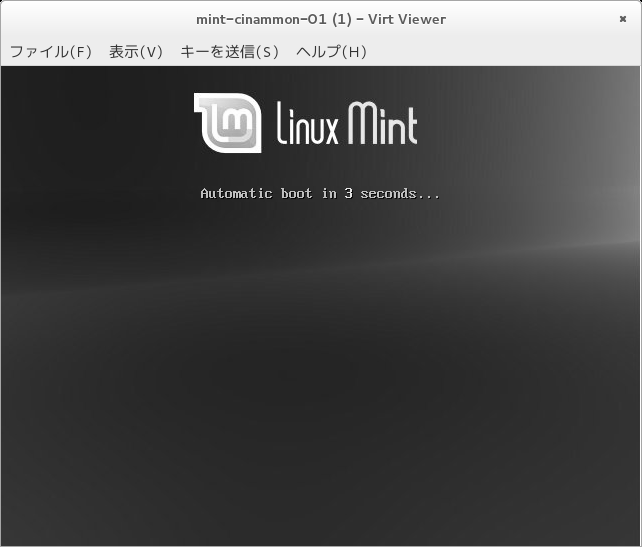
\includegraphics[width=0.8\hsize]{image201412/mint-inst-boot_mono.png}
\caption{ブートの様子}\label{fig:mint-boot}
\end{minipage}
\begin{minipage}{0.5\hsize}
\centering
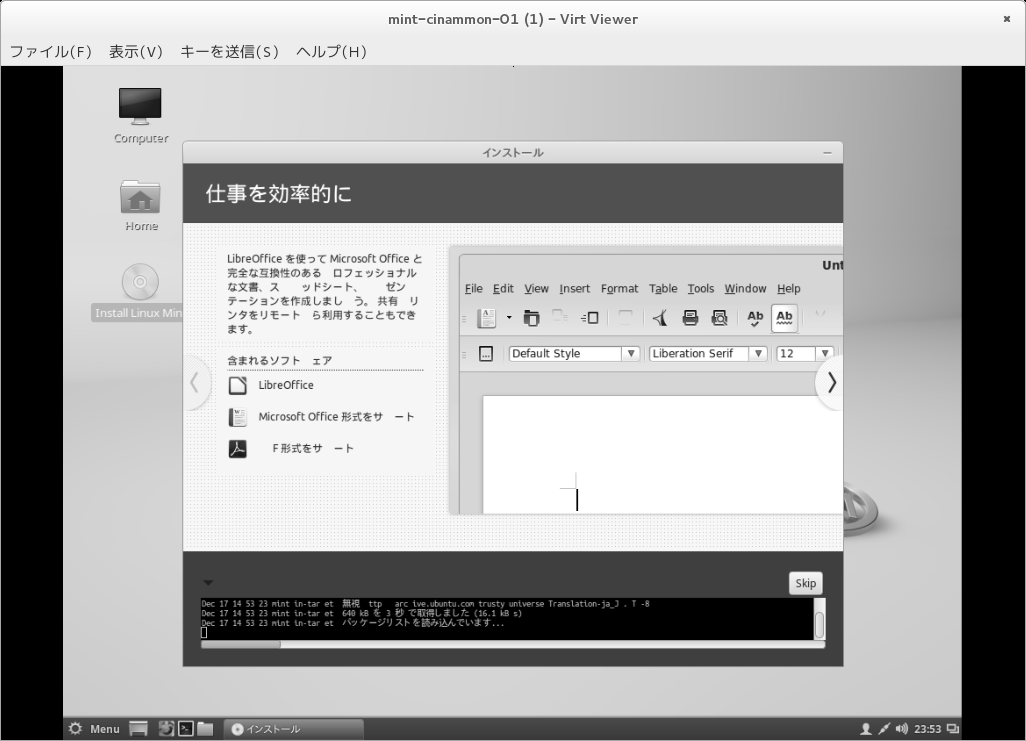
\includegraphics[width=0.8\hsize]{image201412/mint-inst_mono.png}
\caption{インストーラ起動の様子}\label{fig:mint-inst}
\end{minipage}
\end{figure}
\begin{figure}[H]
\begin{minipage}{0.5\hsize}
\centering
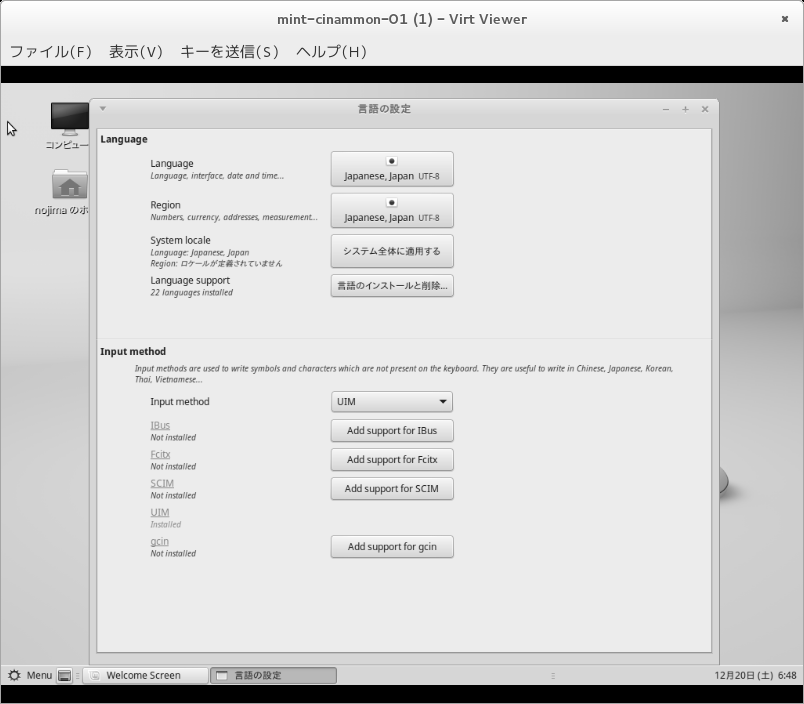
\includegraphics[width=0.8\hsize]{image201412/mint-im-setup_mono.png}
\caption{日本語IM導入の様子}\label{fig:mint-im-setup}
\end{minipage}
\begin{minipage}{0.5\hsize}
\centering
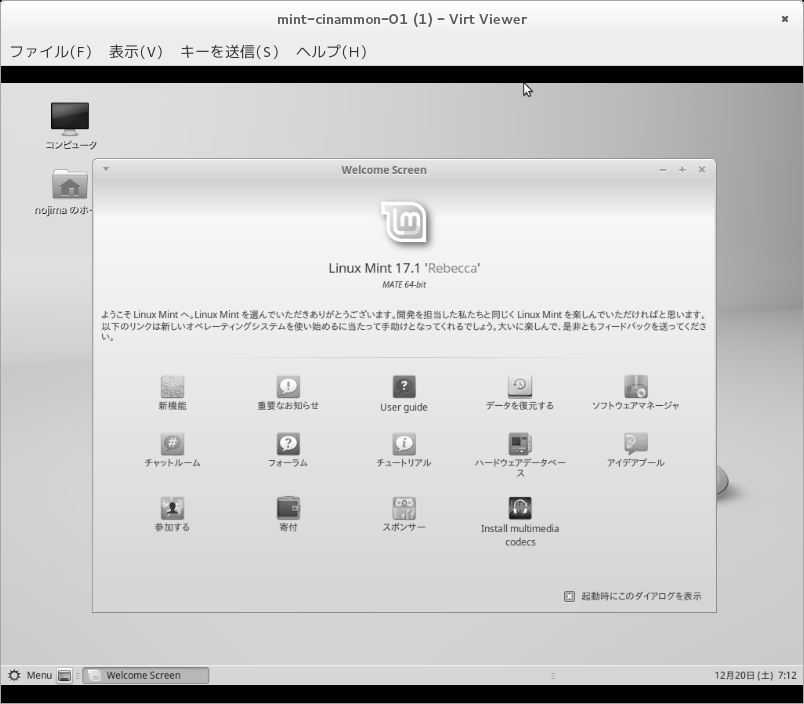
\includegraphics[width=0.8\hsize]{image201412/mint-setupcomplete_mono.png}
\caption{インストール完了}\label{fig:mint-setupcomplete}
\end{minipage}
\end{figure}

 \subsection{Linux MintとUbuntu/Debianの関係}

 図\ref{fig:mint-construct}にLinux MintとUbuntu/Debianの関係を図示しておきます。Linux Mint側ではデスクトップ環境及びMintToolsのみをLinux Mint側で開発しており、残りの足らない部分をすべてUbuntuのパッケージから導入しているという作りとなります。

 このため、パッケージの更新を行う場合、Debianで行うように、うっかりapt-get/aptitudeなどでfull-upgradeすると、Linux Mintでは意図していない形で副作用のあるパッケージがうっかり導入されてしまう事があるため、パッケージの更新の時は「システム管理メニュー」の「アップデートマネージャ」を使ってアップグレードしなければならない等の制約があります。
\begin{figure}[H]
\centering
\includegraphics[width=0.8\hsize]{image201412/mint-construct-mono.eps}  
\caption{Linux MintとUbuntu/Debianの関係}\label{fig:mint-construct}
\end{figure} 

\subsection{Linux Mintの良い所} 

以下にLinux Mintの良い所を載せます。

\begin{itemize}
 \item Linux Mint側でメンテナンスされている部分の作りが非常に丁寧であり、通常の利用であれば、GUIのメニューを操作するだけですぐに使えるのが良い点です。他ディストリビューション(Debian含む)のようにメニューの各項目の動作が不完全、あるいはメニューの項目が不完全ということは非常に少ないように思えます。
 \item Linux Mint側のcommunityサイト\footnote{\url{http://community.linuxmint.com/}}には、投票システムや、ユーザの投稿のランキングなどの様々な統計がすぐにみれるようになっています。さらに、アイデアの投稿場所があり、こちらに投稿されたアイデアについて、他のユーザが好感度を投票でき、どのアイデアが他のユーザに評価が高いかがすぐにわかるようになっています。
\end{itemize}

\subsection{cinnamonをDebian unstableに導入してみる}

 2014/9/4にDebianのtestingにLinux Mintで利用されている
デスクトップ環境であるcinnamonが入ったとのアナウンスがありました。

 ひょっとして、Debianにcinnamonを入れると、Linux Mintそっくりになったりするのかも?と思い、試しにDebian sidへ導入してみました。

\begin{description}
\item [Step 1.] Debian sidをデスクトップ環境を全く導入しない最小限の構成で導入します。
\item [Step 2.] cinnamonデスクトップ環境を導入します。
  \begin{commandline}
$ sudo aptitude install cinnamon-desktop-envirionment
  \end{commandline}
\item [Step 3.] Debina sidをリブートします。すると、lightdmが立ち上がり、ログイン画面が現れます。
\item [Step 4.] ログインすると、Debianらしいルックアンドフィールでcinnamonのディスクトップ環境が動作します。(図\ref{fig:debian-cinnamon})
\end{description}

 使うとわかるのですが、Debianの他デスクトップ環境の完成度としては普通の完成度です。Debianに慣れているのであれば、Debianで導入出来る他デスクトップ同様、管理の流儀も利用も全く違和感がありません。しかしながら、Linux Mintで提供されている程の、システム全体との統合はメニュー構成も含めて実現出来ていない状況です。このため、仮にLinux MintユーザがDebianへ乗り換えることを考えた場合、Debianにcinnamonを導入してみても、物足りなさを感じてしまうかも?と思いました。

\begin{figure}[H]
\centering
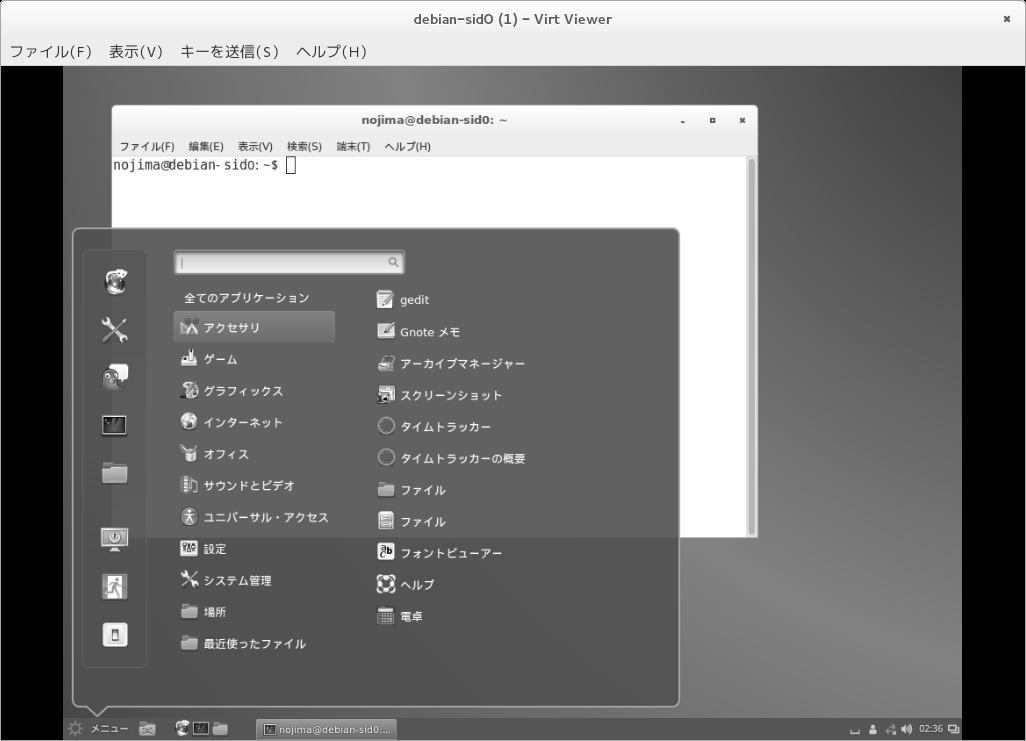
\includegraphics[width=0.6\hsize]{image201412/debian-cinnamon_mono.png}  
\caption{Debianにcinnamonを導入した様子}\label{fig:debian-cinnamon}
\end{figure} 

\subsection{おわりに}

 今回は、Linux MintについてDebianからの視点で見てみました。Linux Mint communityのサイト、Linux Mint並にGUIとシステム管理が丁寧に統合されたデスクトップ環境の構成はDebianを考える上で非常に参考になります。将来こういった点をDebianで導入・改善していくと良いと思いました。

\begin{thebibliography}{9}
\bibitem{ref:linuxmint-history} Linux Mint UserGuide中 Historyの章,\url{http://www.linuxmint.com/documentation/user-guide/MATE/english_4.0.pdf}
\bibitem{ref:linuxmint-illeagal-prog} 「Linux Mintのミラーを再開しました」,\url{http://ftp-admin.blogspot.jp/2013/06/linux-mint.html}
\bibitem{ref:kde-devel-debian}「Debian開発者のKDE環境あれこれ」 第85回東京エリアDebian勉強会資料,\url{http://tokyodebian.alioth.debian.org/pdf/debianmeetingresume201202.pdf}
  \bibitem{ref:dnsmasq}「Debianでdnsmasqを使う」 第109回東京エリアDebian勉強会資料,\url{http://tokyodebian.alioth.debian.org/pdf/debianmeetingresume201402.pdf}
\end{thebibliography}

%201503tokyo
%-------------------------------------------------------------------------------
\dancersection{Raspberry Pi 2 Model B に Debian Jessie / armhf をインストールする}{岩松 信洋}
%-------------------------------------------------------------------------------
 \subsection{はじめに}

2015年2月2日に新しいRaspberry Pi「Raspberry Pi 2 Model B」が発売されました。
今回のRaspberry Pi 2(以下、RPi2)は今までのRaspberry Pi(RPi)とは異なり、SoC がアップグレード
されたものになっています。FPU を持っているにも関わらず Debian では armel をつかわなければ
なりませんでしたが、RPi2ではDebianのarmhf アーキテクチャが利用できるようになります。

本資料では Debianから見たRPi と RPi2 の違いと、RPi2 に Debian Jessie / armhf をインストール
する方法について紹介します。

\subsection{RPi と RPi2 の違い}

\begin{figure}[htbp]
\begin{center}
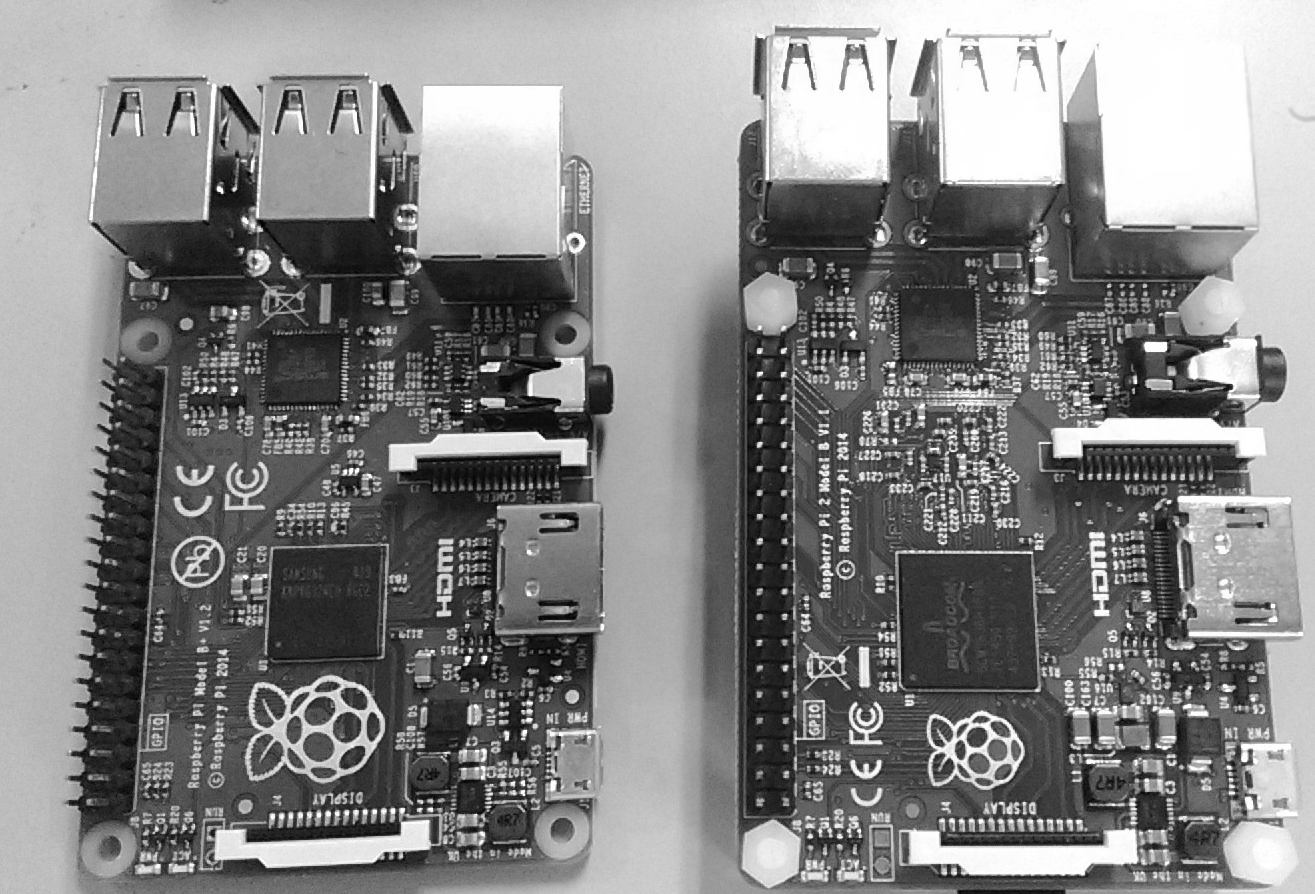
\includegraphics[width=0.7\hsize]{image201503/rpis_mono.png}
\end{center}
\caption{RPi Model B+(左) とRPi 2 Model B(右)}
\label{fig:rpis}
\end{figure}

RPi (Model B+) とRPi 2 Model B のハードウェアは
表\ref{fig:rpi-hw}となります。CPU、コア数、メモリの種類とサイズが大きく異なる
事が分かります。RPi2 ではコア数が増えているため、電源も大きめのものが必要
になっていることも注目すべき点です。
\begin{table}
\caption{RPi とRPi 2 B}
\begin{center}
\begin{tabular}{|c|c|c|}
\hline
-   & RPi Model B+ & RPi 2 Model B \\
\hline
CPU  & ARM1176JZF-S 1コア (700MHz) / ARMv6 & ARM Cortex-A7 4コア (900MHz) / ARMv7\\
SoC  & Broadcom BCM2835 &  Broadcom BCM2836 \\  
CPU  & Broadcom VideoCore IV (250MHz) & 同左 \\
メモリ & 512MB (SDRAM)& 1GB (LPDDR2 SDRAM) \\
ネットワーク & LAN9514 (10/100 Mbps) & 同左 \\
外部I/O & GPIO 40ピン & 同左 \\
ストレージ & microSD & 同左 \\
電源 & 600 mA (3.0W) & 900 mA (4.5-5.5W) \\
\hline
\end{tabular}
\label{fig:rpi-hw}
\end{center}
\end{table}

Debian armel、armhf、Raspbian の違いは表\ref{fig:rpi-sw}の通りです。
各アーキテクチャでサポートする命令セットが異なり、Debian armel
では RPi/RPi2 に最適化されているとは言えないことがわかります。
Unixbench でベンチマークした結果を表\ref{fig:rpi-bench}に示します。
RPi では Raspbian のよい結果となり、RPi2 では Debian / armhf が
よい結果となります。これは Raspbian が ARMv6 / VFPv2 に最適化
されたバイナリで、RPi2 に最適化されていないためです。
RPi2 では Raspbian より Debian / armhf を使ったほうが良いことが
わかりました。

\begin{table}
\caption{Debian と Raspbian}
\begin{center}
\begin{tabular}{|c|c|c|c|}
\hline
 - & Debian armel & Debian armhf & Raspbian \\
\hline
ターゲット命令セット &  ARMv4 & ARMv7 & ARMv6 \\
FPU &  なし &  VFPv3  &  VFPv2 \\
Debian ネイティブ & Yes & Yes & No \\
\hline
\end{tabular}
\end{center}
\label{fig:rpi-sw}
\end{table}

\begin{table}
\caption{UnixBenchの結果}
\begin{center}
\begin{tabular}{|c|c|c|c|c|}
\hline
 - & Debian armel/RPi & Debian armhf/RPi2 & Raspbian/Rpi & Raspbian/Rpi2 \\
\hline
System Benchmarks Index Score & 66.5 & 450.8 (183.1) & 80.1 & 442.9 (173.8)\\
\hline
\end{tabular}
\end{center}
\label{fig:rpi-bench}
\end{table}


\subsection{Debian armhf / Jessie のインストール方法}

インストールには 実機、初期化されてもよい4GB以上のmicroSDカード、電源用の
micro USB ケーブル等が必要です。
またUSBシリアル変換モジュールがあるとコンソールから操作できるので、カスタマイズ
が楽にできます。接続例を図\ref{fig:rpi2-hw-setting}に示します。

\begin{figure}[htbp]
\begin{center}
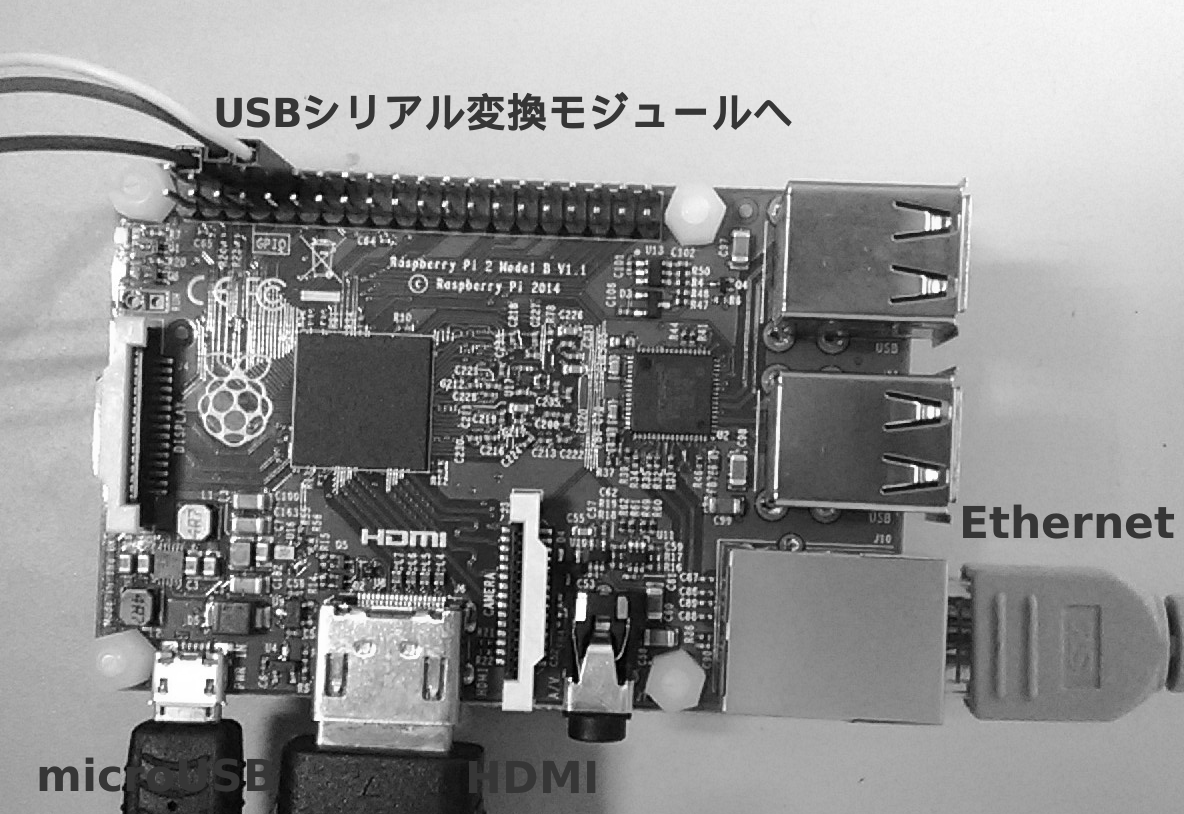
\includegraphics[width=0.7\hsize]{image201503/rpi2-hw-setting_mono.png}
\end{center}
\caption{RPi2 接続例}
\label{fig:rpi2-hw-setting}
\end{figure}

またインストールの流れは以下となります。
\begin{enumerate}
\item microSDカードの認識確認
\item microSDカードの初期化
\item microSDカードにパーティション作成
\item microSDカードのフォーマット
\item cdebootstrap を使ってmicroSDカードにインストール
\item RPi2のLinuxカーネルとカーネルモジュールのインストール
\item RPi2のカーネルコマンドラインの設定
\item fstabの設定
\item ネットワークデバイスの設定
\item rootfs用パーティションの変更
\item root のパスワードの設定とrpiユーザの追加
\item microSDカードのアンマウントとRPi2の起動
\item RPi2 へのログイン
\item RPi2 専用ツールのインストール
\end{enumerate}

\subsubsection{microSDカード の接続確認}

使用している Debianに micorSD カードを挿入します。挿入するとdmesgに以下のような
メッセージが出力されるはずです。これでmicroSDがどのデバイスファイルに割り当てられた
かわかります。図\ref{fig:microsd}では sde に割り当てられていることがわかります。

\begin{figure}[htbp]

\begin{commandline}
$ dmesg  | tail -5
[858983.896718] FAT-fs (sdf1): Directory bread(block 32775) failed
[858983.896729] FAT-fs (sdf1): Directory bread(block 1390704) failed
[858983.896731] FAT-fs (sdf1): Directory bread(block 1390705) failed
[869873.800361] sd 6:0:0:3: [sde] 15523840 512-byte logical blocks: (7.94 GB/7.40 GiB)
[869873.831121]  sde: sde1
\end{commandline}
\caption{microSDカードのデバイスファイル割り当て確認}
\label{fig:microsd}
\end{figure}

\subsubsection{microSDカードの初期化}

購入したばかりのmicroSDカードはVFAT等でフォーマットされています。
MBRがある領域を 0 で埋めて初期化します(fdisk コマンド等で丁寧にやってもよいです)。

\begin{figure}[htbp]
\begin{commandline}
$ sudo dd if=/dev/zero of=/dev/sde bs=1M count=1
\end{commandline}
\caption{microSDカードの初期化}
\label{fig:microsd-format}
\end{figure}

\subsubsection{microSDカードにパーティション作成}

fdisk コマンドを使って microSD カードにパーティションを作成します。
図\ref{fig:createp}に手順を示します。
32MB、VFATで boot 用のパーティションを作成し、残りをrootfs 用にLinux 用に作成します。

一気にやりたい方は図\ref{fig:createp2} を実行すればよいです。

\begin{figure}[htbp]

\begin{commandline}
$ sudo fdisk /dev/sde
Command (m for help): o

Created a new DOS disklabel with disk identifier 0x9aa4e1fa.

Command (m for help): n
Partition type
   p   primary (0 primary, 0 extended, 4 free)
   e   extended (container for logical partitions)
Select (default p): p
Partition number (1-4, default 1): 1
First sector (2048-15523839, default 2048): 
Last sector, +sectors or +size{K,M,G,T,P} (2048-15523839, default 15523839): +32M

Created a new partition 1 of type 'Linux' and of size 32 MiB.

Command (m for help): t
Selected partition 1
Hex code (type L to list all codes): e
If you have created or modified any DOS 6.x partitions, please see the fdisk documentation for additional information.
Changed type of partition 'Linux' to 'W95 FAT16 (LBA)'.

Command (m for help): n
Partition type
   p   primary (1 primary, 0 extended, 3 free)
   e   extended (container for logical partitions)
Select (default p): p
Partition number (2-4, default 2): 2
First sector (67584-15523839, default 67584): 
Last sector, +sectors or +size{K,M,G,T,P} (67584-15523839, default 15523839): 

Created a new partition 2 of type 'Linux' and of size 7.4 GiB.

Command (m for help): w
The partition figure has been altered.
Calling ioctl() to re-read partition figure.
Syncing disks.
\end{commandline}

\caption{microSDカードにパーティションを作成}
\label{fig:createp}
\end{figure}

\begin{figure}[htbp]
\caption{microSDカードにパーティションを作成 一気にやるバージョン}
\begin{commandline}
(echo o; echo n; echo p; echo 1; echo ; echo +32M; echo t; echo e; echo n; echo p; echo 2; echo ; echo ; echo w) | fdisk /dev/sde
\end{commandline}
\label{fig:createp2}
\end{figure}

\subsubsection{microSDカードのフォーマット}

パーティション1 は mkfs.msdos で、パーティション2 は mkfs.ext でフォーマットします。
フォーマットできたら適当なディレクトリを作成し、2つのパーティションをマウントします。
今回は パーティション1用に /tmp/boot ディレクトリ、パーティション2用
に/tmp/rootfs ディレクトリを作成し、マウントします。

\begin{figure}[htbp]
\begin{commandline}
$ sudo mkfs.msdos /dev/sde1
$ sudo mkfs.ext4 /dev/sde2
$ mkdir /tmp/boot /tmp/rootfs
$ sudo mount /dev/sde1 /tmp/boot
$ sudo mount /dev/sde2 /tmp/rootfs
\end{commandline}
\caption{microSDカードのフォーマットとマウント}
\label{fig:microsdformat}
\end{figure}

\subsubsection{cdebootstrap を使ってmicroSDカードにインストールする}

cbootstrap を使って、microSDカードに debian 起動イメージをインストールします。
操作しているマシンがPC(i386やamd64)の場合、通常はarmhf
のバイナリを実行できません。そのためPC等で先にインストールに必要なDebianパッケージのダウンロード
と展開を行い、実際のインストールは RPi2 で行うという方法を取ります。
実際のインストール方法は図\ref{fig:firstbootstrap}となります。今回のインストールでは standard で
指定されているパッケージの他、シリアルコンソールが使えない環境を考えopenssh-server、
時間設定のためにntp、証明書のためにca-certificates、エディタとしてvimをインストールするようにして
います。もし他に一緒にインストールしたいパッケージがある場合は {\bf $-$$-$include} に続けて指定する事ができます。

\begin{figure}[htbp]
\begin{commandline}
$ sudo cdebootstrap --arch=armhf -f standard --foreign jessie \
  --include=openssh-server,ntp,ca-certificates,vim /tmp/rootfs
...
\end{commandline}
\caption{cdebootstrapを使ったDebianイメージのインストール}
\label{fig:firstbootstrap}
\end{figure}

\subsubsection{RPi2のLinuxカーネルとカーネルモジュールのインストール}

残念なことにRPi2のLinuxカーネルはDebianでは提供されていません。その理由として
まだ完全にアップストリームでサポートされていない事と起動にファームウェアが
必要ということが挙げられます。Debianで RPi2 のLinuxカーネルを扱うにはrpi-update
というツールを使う必要があります。

図\ref{fig:kernelinstall}ではrpi-update をRPi2 のrootfs にダウンロードした後、
実行権限を付加し、rpi-update を使ってカーネルとカーネルモジュールをインストールします。

\begin{figure}[htbp]
\begin{commandline}
$ sudo curl -o /tmp/rootfs/usr/bin/rpi-update https://raw.githubusercontent.com/Hexxeh/rpi-update/master/rpi-update
$ sudo chmod +x /tmp/rootfs/usr/bin/rpi-update
$ sudo mkdir /tmp/rootfs/lib/modules
$ sudo ROOT_PATH=/tmp/rootfs BOOT_PATH=/tmp/boot /tmp/rootfs/usr/bin/rpi-update
*** Raspberry Pi firmware updater by Hexxeh, enhanced by AndrewS and Dom 
 *** Performing self-update
  % Total    % Received % Xferd  Average Speed   Time    Time     Time  Current
                                 Dload  Upload   Total   Spent    Left  Speed
100  8107  100  8107    0     0  54471      0 --:--:-- --:--:-- --:--:-- 54777
 *** Relaunching after update
...
\end{commandline}
\label{fig:kernelinstall}
\caption{rpi-updateのインストールとLinuxカーネルのインストール}
\end{figure}

\subsubsection{RPi2のカーネルコマンドラインの設定}

RPi2のカーネルコマンドラインを設定します。RPi は/boot/cmdline.txt
に記載されているカーネルコマンドラインを読み込んで起動します。
図\ref{fig:commandlineset}のように実行し、カーネルコマンドラインを設定します。

\begin{figure}[htbp]
\begin{commandline}
$ sudo sh -c "echo dwc_otg.lpm_enable=0 console=ttyAMA0,115200 console=tty1
     root=/dev/mmcblk0p2 rootwait > /tmp/boot/cmdline.txt
\end{commandline}
\label{fig:commandlineset}
\caption{カーネルコマンドラインの設定}
\end{figure}

\subsubsection{fstabの設定}

fstabの設定を行ないます。procfs、rootfs, boot ディレクトリの設定を記載します。

\begin{figure}[htbp]
\begin{commandline}
proc            /proc           proc    defaults	0	0
/dev/mmcblk0p1  /boot           vfat    defaults	0	2
/dev/mmcblk0p2  /               ext4    defaults,noatime	0	1
\end{commandline}
\label{fig:rpiconfig}
\caption{fstabの設定}
\end{figure}

\subsubsection{ネットワークデバイスの設定}

rootfs/etc/network/interfaces を編集し、ネットワークデバイスを有効にします。
この操作は必須ではありませんが、USBシリアル変換モジュールを持ってない人
はRPi2 にSSHでログインして操作する必要がありますので、ここでネットワークを
起動時に有効するように設定しておきます。
RPi2 のIPアドレスをDHCPから取得する場合は図\ref{fig:netinterfaces}のように設定します。

\begin{figure}[htbp]
\begin{commandline}
auto eth0
iface eth0 inet dhcp
\end{commandline}
\label{fig:netinterfaces}
\caption{ネットワークデバイスの設定}
\end{figure}

\subsubsection{rootfs用パーティションの変更}

rootfs/sbin/init に書かれている 2nd bootstrap の内容に
rootfs をマウントする行があります。デフォルトでは rootfs を / にマウントする
よう記述されているため、このままではインストールに失敗します。
正しくインストールできるように rootfs を /dev/mmcblk0p2 に変更します。

\begin{figure}[htbp]
\begin{commandline}
trap 'error "Interruped!"' HUP INT TERM

mount -n -o remount,rw rootfs / <- これを
mount -n -o remount,rw /dev/mmcblk0p2 / <- これに変更

chown -hR 0:0 /
\end{commandline}
\label{fig:rpiconfig}
\caption{ネットワークデバイスの設定}
\end{figure}

\subsubsection{root のパスワードの設定とrpiユーザの追加}

現状のままではインストール完了後にログインできません。
2nd bootstrap 時にroot のパスワードを設定する処理を追加します。
また rpiユーザを作成し、パスワードを設定する処理も追加します。
rpi ユーザは説明のために使っているだけですので、他のユーザ名でも問題ありません。

\begin{figure}[htbp]
\begin{commandline}
echo 'deb http://ftp.debian.org/debian jessie main' > /etc/apt/sources.list

echo "root:root" | chpasswd <- この行を追加
useradd -m rpi <- この行を追加
echo rpi:rpi | chpasswd <- この行を追加

run rm /sbin/init
\end{commandline}
\label{fig:rpiconfig}
\caption{root パスワードの設定}
\end{figure}

\subsubsection{microSDカードのアンマウントとRPi2の起動}

microSDカードをアンマウントし、PRi2 の microSDカードスロット
に挿入します。挿入後、micro USB ケーブルを RPi2 に挿し、
RPi2を起動します。起動すると自動的に2nd bootstrap が実行され、
RPi2上でインストールが実行されます。
もしHDMI接続ができるモニターを持っている場合は、RPi2 と接続すると
インストールされる様子を確認できます。
インストール完了まで30分ほど待たされるので、気長に待ちましょう。
HDMIが利用できるモニターを持ってない場合、インストールが完了したか
見た目ではわからないので、RPi2 にIPアドレスが割り当てられているか、ping を
実行して反応があるかなどで確認する必要があります。

\subsubsection{RPi2 へのログイン}

インストールが完了すると自動的に init が再実行され、Debian が立ち上がった状態になっています。
USBシリアルモジュール経由や、SSH経由でログインできるようになっていますので、ログインして
ください。後は通常のDebianと変わりません。

\subsubsection{RPi2 専用ツールのインストール}

RPi2 の専用ツールである rpi-update、raspi-config はまだDebianでは提供されていません。
これらはカーネルやファームウェアのアップデート、RPiハードウェアの設定を行うための機能が
搭載されており、RPi ユーザには必須のツールとなっています。
これを Debian で利用できるようにするには raspberrypi.org で提供されている 各ツールの
Debian パッケージをインストールする必要があります。
図\ref{fig:rpirep}に設定方法を示します。

\begin{figure}[htbp]
\begin{commandline}
# wget -O - http://archive.raspberrypi.org/debian/raspberrypi.gpg.key | apt-key add - 
# echo deb http://archive.raspberrypi.org/debian wheezy main >> /etc/apt/sources.list
# apt-get update
# apt-get install rpi-update raspi-config
\end{commandline}
\label{fig:rpirep}
\caption{rpi-config、rpi-update パッケージのインストール方法}
\end{figure}

\subsubsection{終わりに}

RPi2 から ネイティブのDebianが利用できるようになりました。
インストーラやmicroSDカードイメージが準備されていなくても、今回解説した方法を使うと
RPi2 に自分好みのDebianをインストールできるようになります。CPUも強化されそこそこ使い
やすくなった Rpi2 で Debianを触ってみてはいかがでしょうか。

%201505tokyo
%-------------------------------------------------------------------------------
\dancersection{自然言語処理チーム(pkg-nlp-ja)とパッケージ}{野首 貴嗣}
%-------------------------------------------------------------------------------

\subsection{NOTICE}
 私は専門家ではありません。

\subsection{pkg-nlp-ja}
 Debianにおける自然言語処理パッケージの管理
 \url{https://alioth.debian.org/projects/pkg-nlp-ja/}

\subsection{管理パッケージ}
\begin{itemize}
\item ChaSen
\begin{itemize}
  \item dirts (Double Array実装)
\end{itemize}
\item 辞書
\begin{itemize}
\item ipadic
\item naist-jdic
\item unidic
\end{itemize}
\end{itemize}

\subsection{その他のNLPパッケージ}
\begin{itemize}
\item 解析
  \begin{itemize}
  \item MeCab
  \item Juman
  \end{itemize}
\item 変換
  \begin{itemize}
  \item Anthy (pkg-anthy)
  \item KAKASI
  \item mozc
    \begin{itemize}
    \item 変換についてはpkg-imeで管理
    \end{itemize}
  \end{itemize}
\end{itemize}

\subsection{何ができるか}
形態素解析
\begin{itemize}
\item 形態素(単語)を調べる
\item 単語の属性情報を得る
  \begin{itemize}
  \item 品詞・読み等
    \begin{itemize}
    \item 辞書に依存
    \end{itemize}
  \end{itemize}    
\end{itemize}

 ChaSen, MeCab, Juman
 ref:\url{http://www.phontron.com/nlptools.php?lang=ja}

\subsection{応用例}
\begin{itemize}
\item 検索エンジン
  \begin{itemize}
  \item 転地インデックスの作成
  \item Groonga, Namazu等
  \end{itemize}
\item 音声合成 (Text-to-Speech)
  \begin{itemize}
  \item open-jtalk
  \end{itemize}
\item 分かち書き
  \begin{itemize}
  \item word2vecの下処理
  \end{itemize}
\item かな漢字変換
\end{itemize}

\subsection{動作原理}

\begin{itemize}
\item 解析対象を確からしい単位で分割
  \begin{itemize}
  \item 例: 「東京都府中市」
    \begin{itemize}
    \item x 「東」「京都」「府」「中」「市」
    \item o 「東京」「都」「府中」「市」
    \end{itemize}
  \item 単純なルールでは処理できない
  \end{itemize}
\end{itemize}

\subsection{解析の手がかり}

\begin{itemize}
\item マッチする単語の長さ
  \begin{itemize}
  \item 最長一致(KAKASI)
  \end{itemize}
  ref: KAKASIの実装と課題
\item 品詞情報の利用
  \begin{itemize}
    \item 前後に来やすい品詞のつながり
    \item  単語のつながり
    \item  単語の頻度/スコア
  \end{itemize}
\item 確率
  \begin{itemize}
  \item 出現率、連接確率
  \end{itemize}
\end{itemize}

\subsection{アルゴリズム}

\begin{itemize}
\item コスト最小法
  \begin{itemize}
  \item ChaSen
  \end{itemize}
\item CRF (条件付き確率場)
  \begin{itemize}
  \item MeCab
  \end{itemize}
\end{itemize}
ref: 日本語形態素解析入門(pdf)

\subsection{辞書探索}

 Common Prefix Search
\begin{itemize}
 \item 同じ接頭語を持つデータを高速に検索
\end{itemize}  

アルゴリズム
\begin{itemize}
\item トライ
 \begin{itemize}
  \item パトリシアトライ
 \end{itemize}
 \item Double Array
   \begin{itemize}
   \item dartsパッケージ
   \end{itemize}
\end{itemize}

\subsection{トライ(Trie)}

文字単位の木構造

\begin{verbatim}
 漢-+->字-+->化
   |   |
   |     +->語
   +->音
\end{verbatim}

ref: \url{http://ja.wikipedia.org/wiki/基数木}

\subsection{Double Array}

 トライ構造を2つの配列で表現

\begin{itemize}
\item BASE配列 (子ノード番号へのオフセット)
\item CHECK配列 (親ノード番号)
  \begin{itemize}
  \item 単純な状態遷移表だと疎な配列になる
  \item 構築に計算が必要
    \begin{itemize}
    \item 配列の空き要素を見つける必要がある
    \item 動的な更新には向かない
    \end{itemize}
  \end{itemize}
\end{itemize}
ref: ダブル配列の実装方法

\subsection{辞書}

\begin{itemize}
\item KAKASIDIC(kanwadic)
  \begin{itemize}
  \item SKKDICベース
  \end{itemize}
\item ipadic
  \begin{itemize}
  \item ChaSen, MeCab
  \end{itemize}   
\item naist-jdic
  \begin{itemize}
  \item ChaSen, MeCab
  \end{itemize}    
\item jumandic
  \begin{itemize}
  \item MeCab, JUMAN
  \end{itemize}    
\end{itemize}

\subsection{単語の追加: KAKASI}

辞書ファイルの作成(EUC-JP)
\begin{commandline}
# よみ [空白] 漢字
けいさんしょう 経産省
けいざいさんぎょうしょう 経済産業省
\end{commandline}
kakasiコマンドの引数に辞書のパスを追加
\begin{commandline}
$ echo '日本の経産省 ' | kakasi -w -iutf8 -outf8 ./extdic
日本 の 経産省
$ echo '日本の経産省 ' | kakasi -w -iutf8 -outf8
日本 の 経 産 省
\end{commandline}

\subsection{単語の追加: ChaSen}

\begin{itemize}
\item ipadicのソースを取得
\item 追加したい単語の意味に近いものを探す
\item そのエントリーをコピーし、スコアはそのままで単語を修正する
\item ./configure \&\& make 
\end{itemize}
 注: スコアを計算するツールが付属していない

\subsection{単語の追加: MeCab}

\begin{enumerate}
\item ChaSenと同じ方法
  \begin{itemize}
  \item 活用のある品詞はすべて開く必要がある
  \end{itemize}
\item mecab-cost-trainで正確なコストを算出
  \begin{itemize}
  \item 元となるコーパスを用意する必要がある
  \item cf: mecab-ipadic-neologd
  \item MeCab の IPA 辞書を再学習させてみる
  \item MeCabの辞書をカスタマイズする
  \end{itemize}
\end{enumerate}

\subsection{参考}

 自然言語処理ツール\\
\url{http://www.phontron.com/nlptools.php?lang=ja}

 日本語で読める自然言語処理のチュートリアルスライドまとめ\\
\url{http://blog.unnono.net/2015/04/nlp-tutorial.html}

%201504tokyo
%-------------------------------------------------------------------------------
\dancersection{.debから Python パッケージへの変遷}{まえだこうへい}
%-------------------------------------------------------------------------------
\subsection{はじめに}

一昨年\ref{deb}、昨年\ref{debci}、現在の職場で構築および運用している Debian パッケージの自動ビルド\&ローカルアーカイブの仕組みについてお話しました(以下ローカル Debian CI と呼びます)。
昨年後半、部門での開発言語を Python \footnote{Web フレームワークには Django 及び django REST framework に統一しました。}にするという方針になり、同様の形でローカル PyPI を利用した Python パッケージ配布の仕組みを構築しました(以下 ローカル PyPI CI と呼びます)。
今まで運用して分かったメリット/デメリットや、ローカル Debian CI を必要とするケースなどについて紹介します。そして私自身が主に Python 関連の Debian パッケージをメンテナンスしていますが、これに絡めた考察を行います。

\subsection{ローカルDebian CI}

ローカル Debian CI は、git-buildpackage で管理している Git リポジトリもしくはソースパッケージを取得してビルドを行います。前者はインハウスで開発したソフトウェア、後者はバックポートする場合です。git-buildpackage / cowbuilder でのビルド、lintian でのポリシーチェック、piuparts でのインストール/アンインストールテスト、debsign\footnote{実際にはTTYなしでdebsignを実行できないため、Pythonで pydebsignを実装し、使用しています。\ref{pydebsign}}での署名、dput での reprepro へのアップロードを行います。少なくともバックポートに関してはJenkinsのプロジェクトのコピーだけで他のメンバーでも行えます。図\ref{fig:debian-ci}のような構成です。

\begin{figure}[htbp]
  \begin{center}
  \includegraphics[width=0.50\hsize]{image201504/debian-ci.eps}
  \caption{ローカルDebian CI}
  \label{fig:debian-ci}
  \end{center}
\end{figure}

\subsection{ローカル PyPI CI}

ローカル PyPI CI は同様に Jenkins を使用し、repreproに相当するローカル PyPI サーバには devpi \footnote{\url{http://doc.devpi.net/latest/} PyConJP 2014の「パッケージングの今」の資料\ref{pythonpackage}で知りました。} を使用しています。
Jenkinsのジョブスクリプトもやはり Python で実装しました。このスクリプト自体も Python パッケージ化し、ジョブ実行時にローカル PyPI からインストールして実行します。\footnote{ローカルDebian CI用のスクリプトはGitで管理し、ジョブごとにcheckoutする形式でした。}git-buildpackage/cowbuilder でのクリーンビルドに相当するクリーン環境でのテスト実行は Tox を使うことで実現しています。Tox から virtualenv 環境が作られ、Python2.7 / 3.4 でのユニットテスト\footnote{現在のOSはUbuntu Trustyのため、この2バージョンに固定。}、pylint、pychecker でのチェック、Sphinx ドキュメントのビルドのテストを行います。テストが成功するとdevpi-client \footnote{\url{https://pypi.python.org/pypi/devpi-client}、\url{http://doc.devpi.net/latest/userman/devpi_packages.html}} を使い、devpi-server にパッケージのアップロードを行います。

更に、ローカルPyPI CIにはGitHub EnterpriseからのWebhookを使ったジョブの起動と、HipChatへのテスト結果の通知の機能を実装しました。構成は図\ref{fig:pypi-ci}のようになります。

\begin{figure}[h]
  \begin{center}
  \includegraphics[width=0.6\hsize]{image201504/python-ci.eps}
  \caption{ローカルPyPI CI}
  \label{fig:pypi-ci}
  \end{center}
\end{figure}

{\scriptsize
\begin{itembox}[l]{Pythonでの開発環境の標準化}

チームメンバーのスキルレベルもまちまちであるため、品質の底上げのための次のような標準化も行いました。

\begin{itemize}
\item 開発標準化のための指針ドキュメント作成
\item Pythonパッケージのテンプレート化
\item DjangoアプリのPythonパッケージのテンプレート化
\item 独自認証システム用のモック機能付き共通ライブラリやDjangoモジュールの開発、テンプレートへの適用
\item ローカル PyPI CIをローカルの開発環境で使うためのセットアップスクリプトの提供
\item テンプレートおよびローカルPyPI CIの使い方のドキュメント作成、レクチャー
\item HipChatでの主要な変更点の案内、質疑応答
\end{itemize}

テンプレートには次のような機能を予め提供しています。

\begin{itemize}
\item Tox経由でのpytest、pytest-flake、pylint、pycheckerの実行
\item Sphinx automoduleを使ったドキュメントの自動生成、ローカルPyPIへのドキュメントアップロード
\item Djangoベストプラクティスの適用(Djangoプロジェクトのディレクトリ構成、環境ごとのsettings.pyの切替の仕組みなど)や、Djangoおよびdjango REST frameworkを含めたサンプルアプリの提供
\end{itemize}
\end{itembox}}

\subsection{before/after}

\subsubsection{パッケージ化を行えるメンバーの増加}
ローカルDebian CIの構築以前にDebianパッケージの作成のレクチャーを行ったり、ローカルDebian CIの使い方のドキュメントの作成していました。しかし、敷居が高いこともありソースパッケージの作成は他のメンバーが行える状態ではありません。

一方、Pythonパッケージはテンプレートを使い、残りのsetup.pyの必要項目さえ埋めればパッケージ化できます。これによりPythonは書けてもPythonパッケージは作ったことがないメンバーでも簡単にパッケージ化できるようになりました。

\subsubsection{開発時におけるリポジトリの利用の簡易化}
各オフィスビルからや各データセンターから\footnote{オフィスとデータセンター間は基本VPN接続ですが、一部のサービスはHTTPSでアクセスできます。これもその一つです。}でも各リポジトリはアクセスできるので、基本的にはDebianパッケージでもPythonパッケージでもその点は差がありません。しかし、パッケージ化の観点では前者は敷居が高いため、明示的にローカルの開発環境でも使う人は限られていました。\footnote{VMのインストール用のpreseedで設定しているため、知らずに使っている潜在的なユーザ及びサーバは非常に多いです。}
後者はパッケージ化が簡易であることや、アップロードもJenkinsからだけでなく、LDAPアカウントで手元からアップロード可能であり\footnote{devpi-ldap (\url{https://pypi.python.org/pypi/devpi-ldap})というモジュールを利用。}、ローカルPyPIのURLをpipの``\texttt{--index-url}''オプションで指定することで切替可能なため、利用頻度及び明示的な利用ユーザが増加しました。

\subsubsection{パッケージ化のコスト削減}

Debianパッケージでは、基本私一人で行っており独自パッケージをつくるのに掛かる労力は結構かかります。特に依存パッケージが多く、かつそれらが公式パッケージ化されていない場合には大変です。Pythonパッケージの場合には、前述の通り用意したテンプレートを使えばパッケージ化でき、アップロードも簡単であるため、比べるまでもないでしょう。

ただし、Pythonパッケージ以外ではDebianパッケージを作ることも当然あるので、この辺はパッケージを作成できるメンバーを増やす方法を検討する必要があります。\footnote{基本的には最初に公式パッケージ化にすることを検討しています。}

\subsection{ローカルDebian CIが必要なケース}
一方でDebianパッケージのカスタムビルドが必要なケースもまだあります。

\subsubsection{公式パッケージに無い}
まず、Pythonパッケージ以外で、公式パッケージにはないソフトウェアをDebianパッケージ化する場合です。これが一番多いケースです。
理想的にはライセンス上の問題がなければ、公式パッケージ化を目指したいところですが、そこは業務との兼ね合いもあり、コストがかかり過ぎる場合は割りきって、ローカルアーカイブで管理しています。ライセンス上の問題であったり、依存関係が多すぎる場合です。

\subsubsection{公式パッケージにあるがアップストリームのものを使う}

これは社内的な利用実績を重きに置く場合です。他の人が該当システムの主担当でパッケージ化を要望されるとき、アップストリームの配布するバイナリを\texttt{apt-get}でインストール可能にするためにDebianパッケージにしています。\footnote{TomcatとかOracle JDKとか。}
そうすることで外部のリポジトリを登録しなくても、ローカルアーカイブからインストールできるというメリットもあります。\footnote{Cassandraとか。}

自分が主担当の場合には公式パッケージを使うか、Sidからのバックポートを行っています。

\subsubsection{公式パッケージが古すぎて要件を満たさない場合}

この場合はバックポートの場合を行います。UbuntuのLTSやDebianのstable公式パッケージが古く、backportsに存在しないが、Sidやupstreamの配布するソースパッケージがある場合、それを使ってバックポートし、ローカルアーカイブで管理しています。

\subsubsection{Pythonパッケージでの特殊ケース}

これは現時点ではないのですが、OpenStackの導入にあたり、Ansibleで設定を行うよりも、初期のデフォルト設定を加えたカスタムビルドパッケージを使って、インストールとアップデートだけAnsibleで行った方が良いのではないか、という案です。

\subsection{Pythonパッケージの公式Debianパッケージ化について}

最後にPythonパッケージを公式Debianパッケージにすること自体について考えてみます。

\subsubsection{ユーザーの視点}
Debianパッケージとして提供されていると、\texttt{apt-get}でインストールできるのでその点が最大のメリットです。ですので、次のようなものはDebianパッケージになっていると便利です。

\begin{itemize}
\item コマンドラインツール
\item デーモン
\item 上記のパッケージに依存されているライブラリなど(直接ユーザからは見えませんが)
\end{itemize}

\subsubsection{Pythonな人の視点}

Pythonの実行環境と標準ライブラリはシステムパッケージで良いのですが\footnote{pyenvで実行環境そのものも自前で用意する、という人もいるかもしれませんが、私は違うので割愛。}、コードを書くのに使うサードパーティライブラリ自体はpipでインストールできる方が便利です。以前は、Sid上で必要なパッケージの全てをDebianパッケージ化し、Debian stableかUbuntu LTSの本番環境にもそれをバックポートしていました。が、もはや黒歴史となりました。\footnote{当時、ローカルPyPIの存在を知らなかったため、その時点で出来うる方法=Debianパッケージのローカルアーカイブを使いました。PythonパッケージのファイルをHTTPサーバーに置いて公開するというのも管理が面倒ですし。}

DebianパッケージのPythonを使う場合、virtualenv/pyvenvなどvenv環境を作るツールもDebianパッケージを使う方が、環境毎にこれらのインストールをプロジェクトのリポジトリでケアしないですみます。Toxについても下記にある通り、Debianパッケージのpython-toxを使う方が、依存するパッケージによってsetup.pyやtox.iniの記述を変更しないで済みます。


{\scriptsize
  \begin{itembox}[l]{ToxはDebianパッケージのものを使う理由}
  Toxは\texttt{python setup.py test}に統合すれば、\texttt{setup()}の\texttt{install\_requires}に指定したパッケージが\texttt{easy\_install}でローカルにダウンロードされ実行されます。

  しかし、Djangoのように\texttt{pip}しかサポートしないパッケージの場合、\texttt{setup.py test}に統合していても、まず\texttt{easy\_install}でまずローカルにインストールされるのですが、Djangoと関連のパッケージのインストールで失敗します。そのまま再度実行すると、ローカルにインストールされたファイルがあるので、\texttt{setup.py test}からの\texttt{easy\_install}はスキップされ、Toxの実行から始まります。
  ローカルで実行する場合には、これでも良いのですが、Jenkinsなどでジョブ毎にクリーン環境を作る場合、必ず失敗してしまいます。\texttt{setup.py test}に統合したToxではなく、\texttt{tox}コマンドを直接実行する場合、デフォルトでは\texttt{easy\_install}ではなく\texttt{pip}が使われ、パッケージのインストールもtoxinidirの下のtestenvのディレクトリ毎にインストールされるのでこのような問題が発生しません。
\end{itembox}
}

\subsubsection{依存するPythonパッケージに、Debianパッケージを使う場合}

依存するパッケージが既にDebianパッケージ化されている場合は、
\texttt{virtualenv}や\texttt{pyvenv}の\texttt{--system-site-packages}オプションを使えば、DebianパッケージでインストールされたPythonパッケージをvenvに使うこともできます。必要であれば、venv環境内で個別のパッケージのアップデートも可能です。

\subsubsection{開発したWebアプリをDebianパッケージにする場合}

これは公式パッケージというよりは、カスタムビルドが主なケースの話になりますが、Webアプリ自体をDebianパッケージにする場合、\texttt{start-stop-daemon}などでデーモン化し、uWSGI経由でApacheやNginxなどにリバースプロキシする設定をinitスクリプトで用意やれば、ユーザとしてはパッケージのアップデートだけで基本済むので非常に楽です。基本開発が止まっているけど、ソフトウェアそのもの需要があるなら、パッケージにすると便利です。

しかし、Webアプリとして継続的に機能追加し、リリースし続ける場合、パッケージ化するコストが高いということもありますが、一度パッケージ化してしまった後、uscan、uupdateを駆使してDebianパッケージを自動アップデート及びビルドにしたとしても、コミットからリリースまでに手順が増えるので運用に則さないと思われます。良い方法があればぜひ教えてください。\footnote{以前は、ビルド済み配布物の作成に\texttt{bdist\_deb}がありましたが、今は無くなったようです。}

\subsection{Pythonパッケージを公式Debianパッケージにすべきか}
デーモンやコマンドラインツールのパッケージ化であれば、Pythonでないユーザにとってメリットがあるので、パッケージ\&メンテナンスできるならやると良いでしょう。一方、ライブラリだけが目的なら、そもそもPythonでないユーザには使われない上、Pythonな人もpipでインストールするほうが利便性が高いので基本やる必要がないと思います。
一方、C bindingのPythonライブラリの場合、そもそもPyPIに公開されていないこともあります。そういうケースではDebianパッケージは必須になるでしょう。\footnote{例えば、netsnmp-pythonなどはDebianパッケージにしかありません。libvirt-pythonはPyPIにあります。}

Debianパッケージの作り方自体を学ぶのであれば、Pythonは比較的パッケージ化がしやすいのではないかと思います。dh-pythonパッケージに含まれる、\texttt{pybuild}コマンドのおかげで、以前よりもGolangのパッケージ化並に簡単になりました。\texttt{しかし、Golangの方が簡単です。これもあまりパッケージ化する意義が無い言語ですが…。}


ところで以前、PyPIに登録されているPythonパッケージを全部自動でDebianパッケージ化する、という話もあった気がしますが、どこ行ったのでしょうか。

\subsection{まとめ}

基本、Debianパッケージ化するのをやめたら幸せになりました。が、部分的にはDebianパッケージにすることで利便性があがるので、ケースバイケースでやると良いのではないでしょうか、というのが、私の中での結論になっています。
ぜひ、他の方のお考えもお聞かせ頂ければと思います。

そういえば、Rubyでも同じ話が既にされていたと思うのですけど、結局どうなったのでしたでしょうか?

{\scriptsize
\begin{thebibliography}{9}
\bibitem{ref:deb}``とあるWeb企業でのDebianシステムの使い方。``, \url{http://gum.debian.or.jp/2013/session/437.html}
  \label{deb}
\bibitem{ref:debci}``JenkinsでのDebianパッケージ自動化``, \url{http://tokyodebian.alioth.debian.org/2014-07.html}
  \label{debci}
\bibitem{ref:pydebsign}``I made debsign of Python libary that can be run without a TTY``, \url{http://d.palmtb.net/2014/05/28/i_made_debsign_of_python_libary_that_can_be_run_without_a_tty.html}
  \label{pydebsign}
  \bibitem{ref:oraclejdk}``Retrieve and generate debian package of Oracle JDK``, \url{http://d.palmtb.net/2014/04/16/retrieve_and_generate_debian_package_of_oracle_jdk.html}
  \bibitem{ref:debci2}``How to build custom Debian package automatically by Jenkins``, \url{http://d.palmtb.net/2014/04/12/how_to_build_custom_debian_package_automatically_by_jenkins.html}
  \bibitem{ref:tomcat7}``Issue deploying Jenkins to Tomcat7 Debian package in Wheezy``, \url{http://d.palmtb.net/2014/03/27/issue_deploying_jenkins_to_tomcat7_debian_package_in_wheezy.html}
  \bibitem{ref:pythonpackage}``パッケージングの今``, \url{http://www.slideshare.net/aodag/ss-39068785}
    \label{pythonpackage}
\end{thebibliography}
}

%201501tokyo
%-------------------------------------------------------------------------------
\dancersection{Emacs関連パッケージのDebianパッケージ作成}{henrich}
%-------------------------------------------------------------------------------
\index{debian-emacs-package}

\subsection{はじめに}

 Debianでelispパッケージをお作法に従って作る方法について語ってみます。

 emacs関連パッケージのDebianパッケージ化の手続きを簡単にいうと、

\begin{description}
\item [Step 1.] emacsen-commonパッケージを入れる
\item [Step 2.] /usr/share/doc/emacsen-common/debian-emacs-policy.gz を読む
\item [Step 3.] ポリシーに従って作る
\end{description}

以上となります。

…というのも突き放しすぎなので、step by stepで作り方を説明してみます。

\subsection{step by stepでの作り方}

 まず、ソースを展開しておいて、dh-makeパッケージを入れてdh\_makeコマンドでパッケージを作ります。パッケージはdh-make、コマンドはdh\_makeと「-」と「\_」の違いがあるのに注意。この際、*.elなファイルがあるとテンプレートファイルをコピーしてパッケージ名に合わせて修正してくれます(あるいは --with-emacs オプションを使います)。以前は特に.elなファイルがなくてもテンプレートファイルがコピーされていたのですが、毎度消すのが鬱陶しかったのでパッチを送って修正してもらいました(\footnote{\url{http://bugs.debian.org/696793}})

\begin{commandline}
$ sudo apt-get install dh-make
$ dh_make --createorig

Type of package: single binary, indep binary, multiple binary, library, kernel module, kernel patch?
 [s/i/m/l/k/n] s

Maintainer name  : Hideki Yamane
Email-Address    : henrich@XXXXXX
Date             : Sun, 04 Jan 2015 12:26:09 +0900
Package Name     : ag-el
Version          : 0.44
License          : blank
Type of Package  : Single
Hit <enter> to confirm: 
Currently there is no top level Makefile. This may require additional tuning.
Done. Please edit the files in the debian/ subdirectory now. You should also
check that the ag.el Makefiles install into $DESTDIR and not in / .

\end{commandline}
\begin{commandline}
$ ls debian/
README.Debian      changelog  emacsen-install.ex  manpage.sgml.ex  preinst.ex
README.source      compat     emacsen-remove.ex   manpage.xml.ex   prerm.ex
ag.el.cron.d.ex    control    emacsen-startup.ex  menu.ex          rules
ag.el.default.ex   copyright  init.d.ex           postinst.ex      source
ag.el.doc-base.EX  docs       manpage.1.ex        postrm.ex        watch.ex
\end{commandline}

 emacsen-*.ex ファイルがあることがわかります。これをリネームして.exポストフィックスを外してやりましょう。余分なファイルも消しておきます。

\begin{commandline}
$ ls
changelog  control    docs             emacsen-remove   rules   watch
compat     copyright  emacsen-install  emacsen-startup  source
\end{commandline}
%$

 スッキリしました。emacsen* ファイルの中身は特にいじる必要はありません。

 次にdebian/controlを修正します。

\begin{commandline}
$ vi debian/control
------debian/controlファイルここから---------------
Package: ag-el
Architecture: any
Depends: ${shlibs:Depends}, ${misc:Depends}
Description: <insert up to 60 chars description>
 <insert long description, indented with spaces>

Package: ag-el
Architecture: all
Depends: ${shlibs:Depends}, ${misc:Depends}, emacsen-common (>= 2.0.8), emacs,
         silversearcher-ag, 
Description: Emacs frontend to ag
 The Silver Searcher (a.k.a. ag) is very fast grep-like program.
 It is faster and has an attractive features than grep.
 ag.el is simple ag frontend for Emacs, loosely based on ack-and-half.el.
------debian/controlファイルここまで---------------
\end{commandline}
%$

 Architecture: は elisp スクリプトなので all に変えます。ポイントはDepends行のemacsen-common ($>=$ 2.0.8), emacsの2つです。

 emacsen-common ($>=$ 2.0.8)の必要性はEmacs Policyに書いてあります。これと併せてdebian/emacs-compatファイルを置きます(中身は単に「0」とだけする)。このファイルはdh\_installemacsenが処理してくれます。man dh\_installemacsenとすると記載があります。

\begin{commandline}
$ man dh_installemacsen
...中略...
FILES
       debian/package.emacsen-compat
           Installed into usr/lib/emacsen-common/packages/compat/package in the package build directory.
...中略...
\end{commandline}
%$
 
 emacsはメタパッケージになっており、Emacs24などの特定バージョンに依存しています。Depends: emacs24などとすると、Emacs25が出た時に再度Depends行を書き換える必要が発生しますが、このメタパッケージを指定すればパッケージ側での都度変更は不要です。

\begin{commandline}
$ apt-cache show emacs
Package: emacs
Source: emacs-defaults
Version: 46.1
Installed-Size: 25
Maintainer: Rob Browning <rlb@defaultvalue.org>
Architecture: all
Depends: emacs24 | emacs24-lucid | emacs24-nox
Description-ja: GNU Emacs エディタ (メタパッケージ)
 GNU Emacs は、拡張可能で自己説明的なテキストエディタです。
 これは常に推奨の最新 Emacs リリースに依存するメタパッケージです。
Description-md5: 21fb7da111336097a2378959f6d6e6a8
Tag: devel::editor, role::dummy, role::metapackage, suite::emacs, suite::gnu,
 use::editing
Section: editors
Priority: optional
Filename: pool/main/e/emacs-defaults/emacs_46.1_all.deb
Size: 1634
MD5sum: 1f115942065ac452467e02377368ee22
SHA1: dbb1343a3d24f60e5038994e3528dd7486e40943
SHA256: c1fad54e790d69b83f32f2612963baba3ea8091ff3ca72c960c7312096223e3a
\end{commandline}
%$

 その他にもXemacsを含むemacsenというパッケージでの指定もありますが、これは仮想パッケージなので単独で指定はできません。指定するとしたら\texttt{"Depends: emacs | emacsen"} のようにします。

 …とここまで書いて「dh-makeでフォローしてくれればいいんじゃねーの?」と気づきました。では、dh-makeパッケージへのパッチを作りましょう…できましたので、BTSを…しました。将来的にはこの部分は「へーそんなのもあるんだー」的になるはず。あ、reportbugで複数ファイルを添付するには1つずつ-Aで指定が必要なようです。

\begin{commandline}
$ debcheckout dh-make
$ cd dh-make
$ git checkout -b support-modern-emacs-policy
...いろいろ変更...
$ git format-patch master
$ ls
0001-add-emacsen-compat-for-modern-Emacs-lisp-package.patch  0002-add-debian-control-file-for-Emacs-add-on.patch 
debian  dh_make  dh_make.1  lib
$ reportbug -A 0001-add-emacsen-compat-for-modern-Emacs-lisp-package.patch \
-A 0002-add-debian-control-file-for-Emacs-add-on.patch dh-make
\end{commandline}

 これでBug\#774545として登録されました。

 しかし、ここで気になることが。dh-makeでのdebian/controlファイルはどうも種類に合わせてコピーされるようです。これをそのまま適用すると、*.elファイルがある場合に否応なしにEmacs add-onパッケージ用のcontrolファイルになるわけで、複数のバイナリパッケージを生成するような場合には嬉しくありません。

 多分、大本のcontrolファイルがあって、Emacs用のが追加される形のほうが嬉しい…のでは?という気がします。…しかし、その場合の「Section: lisp」指定をどうするのか…

\begin{commandline}
Source: #PACKAGE#
Section: lisp
Priority: optional
Maintainer: #USERNAME# <#EMAIL#>
Build-Depends: #BUILD_DEPS#
Standards-Version: #POLICY#
Homepage: <insert the upstream URL, if relevant>
#Vcs-Git: git://anonscm.debian.org/collab-maint/#PACKAGE#.git
#Vcs-Browser: http://anonscm.debian.org/cgit/collab-maint/#PACKAGE#.git/

Package: #PACKAGE#
Architecture: all
Depends: ${misc:Depends}, emacsen-common (>= 2.0.8), emacs | emacsen,
Description: <insert up to 60 chars description>
 <insert long description, indented with spaces>
\end{commandline}
%$

これ、パッケージのところだけを「追記」する形だといいのですかね?

\begin{commandline}
Package: #PACKAGE#
Section: lisp
Architecture: all
Depends: ${misc:Depends}, emacsen-common (>= 2.0.8), emacs | emacsen,
Description: <insert up to 60 chars description>
 <insert long description, indented with spaces>
\end{commandline}
%$

 そうすればソースパッケージの雛形も1箇所でまとめれば済んで、いい感じになるんじゃないか?とか思い始めました。

\begin{commandline}
Source: #PACKAGE#
Section: UNKNOWN
Priority: optional
Maintainer: #USERNAME# <#EMAIL#>
Build-Depends: #BUILD_DEPS#
Standards-Version: #POLICY#
Homepage: <insert the upstream URL, if relevant>
#Vcs-Git: git://anonscm.debian.org/collab-maint/#PACKAGE#.git
#Vcs-Browser: http://anonscm.debian.org/cgit/collab-maint/#PACKAGE#.git/
\end{commandline}

 でもそれは別ハックですね…。

 あとはdebuildしてlintianのwarningなどをちょこちょこと直せば完成です。

\begin{commandline}
$ dpkg --contents /var/cache/pbuilder/result/ag-el_0.44-1_all.deb 
drwxr-xr-x root/root         0 2015-01-04 13:35 ./
drwxr-xr-x root/root         0 2015-01-04 13:35 ./usr/
drwxr-xr-x root/root         0 2015-01-04 13:35 ./usr/share/
drwxr-xr-x root/root         0 2015-01-04 13:35 ./usr/share/doc/
drwxr-xr-x root/root         0 2015-01-04 13:35 ./usr/share/doc/ag-el/
-rw-r--r-- root/root       175 2015-01-04 13:10 ./usr/share/doc/ag-el/changelog.Debian.gz
-rw-r--r-- root/root      1089 2015-01-04 13:35 ./usr/share/doc/ag-el/copyright
-rw-r--r-- root/root      5279 2014-08-05 05:58 ./usr/share/doc/ag-el/README.md.gz
drwxr-xr-x root/root         0 2015-01-04 13:35 ./usr/lib/
drwxr-xr-x root/root         0 2015-01-04 13:35 ./usr/lib/emacsen-common/
drwxr-xr-x root/root         0 2015-01-04 13:35 ./usr/lib/emacsen-common/packages/
drwxr-xr-x root/root         0 2015-01-04 13:35 ./usr/lib/emacsen-common/packages/remove/
-rwxr-xr-x root/root       465 2015-01-04 13:35 ./usr/lib/emacsen-common/packages/remove/ag-el
drwxr-xr-x root/root         0 2015-01-04 13:35 ./usr/lib/emacsen-common/packages/install/
-rwxr-xr-x root/root      1280 2015-01-04 13:35 ./usr/lib/emacsen-common/packages/install/ag-el
drwxr-xr-x root/root         0 2015-01-04 13:35 ./usr/lib/emacsen-common/packages/compat/
-rw-r--r-- root/root         2 2015-01-04 13:35 ./usr/lib/emacsen-common/packages/compat/ag-el
drwxr-xr-x root/root         0 2015-01-04 13:35 ./etc/
drwxr-xr-x root/root         0 2015-01-04 13:35 ./etc/emacs/
drwxr-xr-x root/root         0 2015-01-04 13:35 ./etc/emacs/site-start.d/
-rw-r--r-- root/root      1225 2015-01-04 13:35 ./etc/emacs/site-start.d/50ag-el.el
\end{commandline}
%$

\subsection{まとめ}

\begin{itemize}
\item elispパッケージは emacsen-common パッケージを入れて /usr/share/doc/emacsen-common/debian-emacs-policy.gz ファイルに従ってパッケージを作ろう
\item お手軽にするにはdh-makeパッケージを使おう
\item Policyを読んでtipsを確認する手間を省くにはdh-makeパッケージをハックしてしまえばいい
\end{itemize}

%201502tokyo
%-------------------------------------------------------------------------------
\dancersection{Debian GNU/kFreeBSDにおけるJail構築を試してみた}{杉本 典充}
%-------------------------------------------------------------------------------
\index{debian-kfreebsd-jail}

\subsection{はじめに}

Debian GNU/kFreeBSDは、FreeBSDカーネルで動作するDebianです。
近頃はdockerを実装例としたコンテナ環境に復権(?!)の兆しがあるようにも思えます。そこで、Debian GNU/kFreeBSDをホストとして、FreeBSD Jail環境の構築を試してみます。

\subsection{Debian PortsとDebian GNU/kFreeBSD}

Debian Ports \footnote{\url{https://www.debian.org/ports/}}とは、さまざまなCPUやカーネルで動作するように移植を行うプロジェクトのことです。

FreeBSDカーネルで起動するDebianを作るプロジェクトがあり、そのDebianのことを「Debian GNU/kFreeBSD」と呼んでいます(kはkernelのこと)。現在ではIntel CPUのアーキテクチャのみあります(kfreebsd-amd64、kfreebsd-i386)。Debian 6 (Squeeze)ではテクノロジープレビューとして初めてstableリリースされました。Debian 7 (Wheezy)でも継続してstableリリースされたのですが、Debian 8 (Jessie)ではDropされることが決まっています。\footnote{\url{https://lists.debian.org/debian-devel-announce/2014/09/msg00002.html}において、stableを維持しつつsidの開発を進めるにはそれなりに人手が必要であるが、kFreeBSDを作業する人手は不足していることが指摘されています。}

\subsection{Debianにおけるコンテナ環境の構築方法}

Debianにおいて、コンテナ環境を構築するにはdebootstrapを使います。通常はホスト環境と同じアーキテクチャを引数に指定して実行します。\footnote{debootstrapについては昔の記事にまとめたものがあります。「debootstrap を有効活用してみよう」\url{http://tokyodebian.alioth.debian.org/pdf/debianmeetingresume2013-natsu.pdf}}

\begin{commandline}
# apt-get install debootstrap
# mkdir -p /srv/jail
# cd /srv/jail
# debootstrap --arch=[arch] [release] [dir] http://ftp.jp.debian.org/debian
\end{commandline}

ホスト環境のアーキテクチャと異なるアーキテクチャのコンテナ環境を用意すると普通は動作しません。
ところが、Debianではコンテナ環境とqemuを組み合わせることでエミュレーション動作させつつ、見た目はコンテナ環境でバイナリを実行させる方法があります。これをCrossDebootstrapと言います。\footnote{\url{https://lists.debian.org/debian-mips/2011/02/msg00031.html} 2011年頃にkfreebsd-mips対応をしていた動きがあるようで、これが動くようになればkFreeBSDでCrossDebootstrapを使える日がくるかもしれません。}

\begin{commandline}
# apt-get install qemu binfmt-support qemu-user-static
# debootstrap --foreign --arch=[arch] [release] [dir] http://ftp.jp.debian.org/debian
# cp /usr/bin/qemu-[arch]-static /[dir]/usr/bin/
# chroot [dir]
# /debootstrap/debootstrap --second-stage
\end{commandline}

\subsection{Debian GNU/kFreeBSDをホストとしたJail環境の構築}

Debian GNU/kFreeBSD上でJail環境を構築してみました。環境は以下で行いました。

\begin{itemize}
  \item ホスト環境 
  \begin{itemize}
    \item Debian GNU/kFreeBSD unstable amd64
    \item FreeBSD-10.1 kernel (10.1~svn274115-2)
  \end{itemize}
  \item ネットワーク環境 
  \begin{itemize}
    \item ホストとコンテナが同一ネットワーク(192.168.0.0/24)
  \end{itemize}
  \item コンテナ環境
  \begin{itemize}
    \item FreeBSD Jailにて起動する
  \end{itemize}
\end{itemize}

jailコマンドはaptでインストールできます。

\begin{commandline}
# apt-get install freebsd-utils
# which jail
/usr/sbin/jail
\end{commandline}

ただし現状では、jls\footnote{jlsは起動しているjailを一覧表示するコマンドです。Jail環境として動作しているコンテナは、kernelによってjidという番号を付与され識別されます。}、jexec\footnote{jexecはJail環境内でコマンドを実行するコマンドです。実行例は 「\# jexec 1 /bin/sh」}コマンドはパッケージ化されていません。そのため、今回はJail環境でsshdを動かし、sshログインできるようにすることをゴールとします。

Jail環境を作成して起動するには以下の作業を行います。

\begin{itemize}
  \item Jail環境の動作に必要なバイナリや設定ファイル等のディレクトリツリーを配置する
  \item ネットワークデバイスにIP Alias設定を行う
  \item Jail環境内の動作に必要な/devやファイルシステムのmountを行う
  \item jailコマンドを実行してJail環境を起動する
\end{itemize}


\subsubsection{kfreebsd-amd64、kfreebsd-i386のJail環境}

ホスト環境と同じアーキテクチャのJail環境を作成します。以下の手順はkfreebsd-amd64を指定していますが、kfreebsd-i386も同様の手順で構築することができます。

\begin{commandline}
# mkdir -p /srv/jail
# cd /srv/jail
# debootstrap --arch=kfreebsd-amd64 wheezy jail_kf64_1 http://ftp.jp.debian.org/debian
\end{commandline}

Jail環境内の設定ファイルを変更します。

\begin{commandline}
# cd /srv/jail
# vi jail_kf64_1/etc/resolv.conf
nameserver 192.168.0.1

# vi jail_kf64_1/etc/hostname
jail_kf64_1
\end{commandline}

Jail環境内でsshdが動くように設定します。

\begin{commandline}
# chroot jail_kf64_1
# apt-get install openssh-server
# passwd
# adduser user
# passwd user
\end{commandline}

Jail環境を起動するにはdebootstrapしたディレクトリをjailコマンドの引数に指定します。DebianのwebサイトにJail環境を起動する前処理を含めたスクリプトの例があります\footnote{\url{https://wiki.debian.org/Debian_GNU/kFreeBSD/Jails}}。複数のJail環境を構築するため、スクリプトと起動パラメータを記述した設定ファイルに分割するよう修正しました。

設定ファイルは以下です。

\begin{commandline}
$ cat jail_kf64_1
#!/bin/sh
JID=1
JID_HOST=jail_kf64_1
JID_IPADDR=192.168.0.61
JID_NETMASK=255.255.255.0
JID_SH_PARAM=''-- -c''
JID_CMD=''/etc/init.d/rc S && /etc/init.d/rc 2''
\end{commandline}

起動スクリプトは以下です。

\begin{commandline}
$ cat jail-bootstrap.sh
#!/bin/sh

. ./$1

echo ``----''
echo ``start prison.''
echo ``[target] JID: $JID, name: $JID_HOST''
echo ``----''
echo

NIC_DEV=em0

# add ip alias
/sbin/ifconfig $NIC_DEV alias $JID_IPADDR netmask $JID_NETMASK


# Linux-like /proc and /sys filesystems
mount -t linprocfs linprocfs /srv/jail/$JID_HOST/proc
mount -t linsysfs linsysfs /srv/jail/$JID_HOST/sys

# Ramdisk required for /run
mount -t tmpfs tmpfs /srv/jail/$JID_HOST/run

# A read-only /dev filesystem with restricted set of devices
mount -t devfs devfs /srv/jail/$JID_HOST/dev
# :XXX: ruleset 4 must be initialised as explained earlier in this Wiki page
devfs -m /srv/jail/$JID_HOST/dev rule -s 4 applyset
# Ensure the jail has some essential devices
for DEVICE in null random urandom zero
do if [ ! -e /srv/jail/$JID_HOST/dev/$DEVICE ]
    then
        echo ``error: device '/dev/$DEVICE' MUST be available in the jail''
        exit 1
    fi
done

# Ensure the jail has only a limited set of devices
#for DEVICE in mem kmem
#do if [ -e /srv/jail/$JID_HOST/dev/$DEVICE ]
#    then
#        echo ``error: device '/dev/$DEVICE' MUST NOT be available in the jail''
#        exit 1
#    fi
#done

# Compatibility symlink from /dev/shm to /run/shm
ln -s /run/shm /srv/jail/$JID_HOST/dev/

# Optionally enable networking
HOSTNAME=$JID_HOST
# :XXX: this IP address *must* be assigned to one of the host's interfaces before the guest can use it
IP=$JID_IPADDR

mkdir -p /var/run/jail
jail -J /var/run/jail/$JID.jid -c jid=$JID \
  name=jail$JID \
  path=/srv/jail/$JID_HOST \
  host.hostname=$JID_HOST \
  ip4.addr=$IP \
  command=/bin/sh $JID_SH_PARAM ``$JID_CMD''
\end{commandline}

スクリプトを実行してJail環境を起動します。

\begin{commandline}
$ sudo ./jail-bootstrap.sh jail_kf64_jail

----
start prison.
[target] JID: 1, name: jail_kf64_1
----

devfs rule: ioctl DEVFSIO_SAPPLY: No such process
[info] Using makefile-style concurrent boot in runlevel S.
hostname: the specified hostname is invalid
kern.module_path: /lib/modules/10.1-0-amd64
sysctl: kern.module_path=/lib/modules/10.1-0-amd64: Operation not permitted
[....] Loading devfs rules...devfs ruleset: ioctl DEVFSIO_SUSE: Operation not permitted
 (warning).
mount: tmpfs: Operation not permitted
mount: tmpfs: Operation not permitted
[ ok ] Activating swap...done.
mount: /: unknown special file or file system
mount: /run: unknown special file or file system
mount: /proc: unknown special file or file system
mount: /sys: unknown special file or file system
[ ok ] Activating lvm and md swap...done.
[....] Checking file systems...fsck from util-linux 2.25.2
done.
[ ok ] Cleaning up temporary files... /tmp.
[ ok ] Mounting local filesystems...done.
/etc/init.d/mountall.sh: 59: kill: No such process

[ ok ] Activating swapfile swap...done.
mount: tmpfs: Operation not permitted
mount: tmpfs: Operation not permitted
[ ok ] Cleaning up temporary files....
[....] Starting device state change daemon : devddevd: Can't open devctl device /dev/devctl: Device or resource busy
 failed!
[....] Configuring network interfaces...ifconfig: up: permission denied
ifconfig: socket(family 28,SOCK_DGRAM: Protocol not supported
done.
[ ok ] Cleaning up temporary files....
[FAIL] startpar: service(s) returned failure: hostname.sh kldutils ... failed!
[info] Using makefile-style concurrent boot in runlevel 2.
[....] Starting enhanced syslogd: rsyslogdln: failed to create symbolic link '/dev/xconsole': Operation not permitted
. ok
[ ok ] Starting periodic command scheduler: cron.
[ ok ] Starting OpenBSD Secure Shell server: sshd.
\end{commandline}

Jail環境へsshログインします。

\begin{commandline}
$ ssh user@192.168.0.61
user@192.168.0.61's password:

user@jail_kf64_1:~$
\end{commandline}

Jail環境内のプロセスをすべて停止したい場合はJail環境内で以下コマンドを実行します。

\begin{commandline}
root@jail_kf64_1:~# sh /etc/init.d/rc 0
\end{commandline}


\subsubsection{FreeBSD-10.1-RELEASEのJail環境}

FreeBSDのディレクトリツリーを取得して展開します。

\begin{commandline}
# mkdir -p /srv/jail/jail_fb101_1
# cd /srv/jail/jail_fb101_1
# wget http://ftp.jaist.ac.jp/pub/FreeBSD/releases/amd64/amd64/10.1-RELEASE/base.txz
# tar xvf base.txz
# ls
COPYRIGHT  bin dev  lib      media  proc    root  sys  usr
base.txz   boot  etc  libexec  mnt    rescue  sbin  tmp  var
\end{commandline}

Jail環境内の設定ファイルを変更します。

\begin{commandline}
# vi etc/resolv.conf
nameserver 192.168.0.1
\end{commandline}

Jail環境内でsshdが動くように設定します。

\begin{commandline}
# vi etc/rc.conf
sshd_enable=''YES''
sendmail_enable=''NONE''

# cd ..
# chroot jail_fb101
# passwd
# adduser user
# passwd user
\end{commandline}

FreeBSD-10.1-RELEASEのJail環境を起動するスクリプトの設定ファイルは以下です。

\begin{commandline}
$ cat jail_fb101_1
JID=3
JID_HOST=jail_fb101_1
JID_IPADDR=192.168.0.63
JID_NETMASK=255.255.255.0
JID_SH_PARAM=''''
JID_CMD=''/etc/rc''
\end{commandline}

Jail環境を起動します。

\begin{commandline}
$ sudo ./jail-bootstrap.sh jail_fb101_1

----
start prison.
[target] JID: 3, name: jail_fb101_1
----

mount: /srv/jail/jail_fb101_1/usr/src/sys: No such file or directory
mount: /srv/jail/jail_fb101_1/run: No such file or directory
devfs rule: ioctl DEVFSIO_SAPPLY: No such process
/etc/rc: WARNING: $hostname is not set -- see rc.conf(5).
Creating and/or trimming log files.
ln: /dev/log: Operation not permitted
Starting syslogd.
ELF ldconfig path: /lib /usr/lib /usr/lib/compat /usr/local/lib
32-bit compatibility ldconfig path: /usr/lib32
Clearing /tmp (X related).
Updating motd:.
Performing sanity check on sshd configuration.
Starting sshd.
Starting cron.

Mon Feb 16 22:43:36 UTC 2015
\end{commandline}

Jail環境へsshログインします。

\begin{commandline}
$ ssh user@192.168.0.63
Password for user@jail_fb101_1:

user@jail_fb101_1:~ %
\end{commandline}

Jail環境内のプロセスをすべて停止したい場合はJail環境内で以下コマンドを実行します。\footnote{\url{https://www.freebsd.org/doc/en/books/handbook/jails-build.html}にそう記述がありプロセスはあらかた停止しているように見えますが、kernelではまだjidが生きているようでゴミが残ってしまうようです。}

\begin{commandline}
root@jail_fb101_1:/ # sh /etc/rc.shutdown
\end{commandline}


\subsubsection{linux-i386のJail環境}

【注意】debianとしては動きませんでしたので、試したところまで述べます。


FreeBSD kernelにはLinuxバイナリ互換機能というものがあり、32bitのLinuxバイナリを動かすことができます。FreeBSDにおいてLinuxバイナリ互換機能を有効にするには、linux\_base Portsをインストールし、linux.koをkldloadします。Debian GNU/kFreeBSDではkernelにstatic linkしていますのでlinux.koのロードは不要でした。

Linuxバイナリ互換機能を動かす場合は、ホスト環境のsysctl設定でlinux kernelのバージョンを指定する必要があります。今回はlinux-2.6.32を採用しているsqueezeにしてみました。\footnote{バージョンが異なった状態でchrootしてコンテナ内のバイナリを実行すると「FATAL: kernel too old」というエラーが発生します。(新しくてもtoo oldのようです)} \footnote{FreeBSD Portsにおいて「linux\_base-c6」が実験的に提供されており、機能はCentOS-6のlinux kernel相当です。CentOS-6のlinux kernelは2.6.32を採用しており、squeezeと同じです。}

\begin{commandline}
# vi /etc/sysctl.conf
compat.linux.osrelease=2.6.32

# sysctl -p /etc/sysctl.conf
compat.linux.osrelease: 2.6.16 -> 2.6.32
\end{commandline}


\begin{commandline}
# mkdir -p /srv/jail
# cd /srv/jail
# debootstrap --foreign --arch=i386 squeeze jail_linux32_1 http://ftp.jp.debian.org/debian
\end{commandline}


chrootでコンテナ環境に入ってみます。コンテナ環境の中でシェルは動きますのでLinuxバイナリ互換機能は動いているようです。

\begin{commandline}
# chroot jail_linux32_1
I have no name!@test-kf2:/# 
\end{commandline}

しかし、debootstrapのsecond-stageでエラーになりました。

\begin{commandline}
I have no name!@test-kf2:/# /debootstrap/debootstrap --second-stage
/debootstrap/debootstrap: 1303: /debootstrap/debootstrap: cannot create //test-dev-null: Operation not supported
E: Cannot install into target '/' mounted with noexec or nodev
\end{commandline}

すんなり動いてはくれない状況です。mount絡みのエラーですので、mountできるようにコンテナの中を設定するか、debootstrapのスクリプトを修正するなど対処すると動くのかもしれません。

今回試せたのはここまででした。

\subsection{おわりに}

Debian GNU/kFreeBSDでFreeBSD Jail環境の構築を試してみました。
Debian GNU/kFreeBSD on FreeBSDの構成でも動作することは確認していますので試してみるのもおもしろいです。\footnote{FreeBSD Portsに/usr/ports/sysutils/debootstrapがあります。}

本家FreeBSDのJailのように便利に利用するツールのパッケージが足りていない状況ですので、Debian GNU/kFreeBSDの開発を進めるとどんどん使いやすくなると思います。

\subsection{参考資料}
\begin{itemize}
  \item Debian/kFreeBSDでjailを使う \url{http://hachulog.blogspot.jp/2011/11/debiankfreebsdjail.html}
  \item Debian\_GNU kFreeBSD Jails  \url{https://wiki.debian.org/Debian\_GNU/kFreeBSD/Jails}
  \item あんどきゅめんてっど でびあん2013年夏号 「debootstrap を有効活用してみよう」 杉本典充 \url{http://tokyodebian.alioth.debian.org/pdf/debianmeetingresume2013-natsu.pdf}
\end{itemize}

%201412kansai
\dancersection{DPNで振り返る2014}{かわだ てつたろう}

2014年に発行されたDPN(Debian Project News\footnote{\url{https://www.debian.org/News/weekly/}})
からDebian Project界隈の動向をざっと振り返ってみたいと思います。

2014年は1月6日号から12月1日号まで計16通発行されました。

\subsection{1st quarter}

1月31日、IA64アーキテクチャがJessieから取り除かれました。

2月11日、CTTEはJessieのLinuxアーキテクチャのinitシステムをsystemdとする決定を行な
いました。

3月19日、Jessieのインストーラのアルファ1をリリースされました。

\subsection{2nd quarter}
4月17日、DPL選挙の結果再選されたLucas NussbaumさんのDPL体制がスタートしました。

4月28日、Code of Conductが批准されました。これは先のCTTEのsystemdの決定を受けて
debian-develメーリングリストが荒れに荒れたことに端を発しています。

4月26日、SPARCアーキテクチャがJessieから取り除かれました。

5月22日、Debian GNU/Hurdの活動報告があり、80\%のパッケージをカバーしSysVinitが動作す
るとのことです。

5月31日、旧stableのSqueezeはサポート終了となりました。しかし、新な試みとして限
定ながら5年の長期サポートを目指して「squeeze-lts」が始まりました。

6月3日、MATE1.8の全パッケージングが完了したとのアナウンスがありました。

6月18日、libcがeglibcからglibcに戻りました。

\subsection{3rd quarter}

8月16日、Debian Dayを迎えDebianは21歳になりました。

8月22日から8月31日にかけてDebConf14がアメリカのオレゴン州ポートランドで開催され
ました。

9月4日、Cinnamonの全パッケージがJessieに入ったと報告がありました。

9月19日、再評価の結果Jessieのデフォルトデスクトップ環境がGNOMEに決まりました。

\subsection{4th quarter}

10月22日、Debian Multimedia Maintainersからの活動報告があり、Codecのアップデート、
新しいアプリの紹介などがありました。

11月5日、Jessieのフリーズが行なわれました。

11月9日、Debian 9のコードネームは"Stretch"でDebian 10のコードネームは"Buster"であ
るとリリースチームより報告がありました。

11月18日、「init system coupling」の投票結果が「General Resolution is not required」
となりました。

\dancersection{2014年の振り返りと2015年の企画}{Debian JP}

2014年も今月で最後の関西Debian勉強会になります。
2007年3月からはじまった勉強会も今年で8年目になり、来年には100回目を迎えようとしています。

\subsection{勉強会全体について}

\subsubsection{もくもくの会}

今年からは内容をもくもくの会を主体として開催するようにしました。
各自抱えておられる作業を持ち寄って進めていくよい場となりました。しかし、参加され
たことのない新規の方々にとっては、内容がよくわからないようで、障壁となってしまっ
た面もあるようです。

\subsubsection{セッション、定例ネタ}

毎回のセッションは設定しませんでしたが、「Debian で楽しむ 3D プリンティング」、
「自宅サーバにkvmを導入してみよう」、「Notmuch Mail」、「Debian での systemd と
  のつきあい方」、「Linuxのドライバメンテナになった体験記」の5本の発表をしていただ
きました。

いわゆる定番のネタについてのセッションはできませんでした。
来年はjessieのリリースにあわせて定番のネタ(Debianの入門的なお話、ライセンス、パッ
ケージ作成、BTS)のセッションができたら良いかなと考えています。

\subsection{運営}

運営に関しては、毎月の継続した開催は行なってきていました。

申し込みのシステムとしてDoorkeeperを試験的に使用しました。
connpassなど他の手段も試し、いわゆる今風の申し込みやすい環境を整えていきます。

昨年に続き、事前の準備、告知が不十分な場合がありましたので、今後は、定型の告知を
先に投げるなど、改善していきたいと考えています。

また、運営に参加していただいていた八津尾さんが、関西から離れられることになり、運
営から抜けられました。

\subsection{イベント/NM申請}

イベント参加については、OSC Kansai@Kyoto、KOF2014に参加しました。
今後も継続して参加する予定です。
%
今年は合宿や「大統一Debian勉強会」などのイベントの実施はありませんでした。

Debian開発者への道、として一昨年から倉敷さんがNMプロセスの申請を進められています。
今後もNMプロセスに挑む参加者やDebian Maintainerとなって精力的にパッケージを開発/
更新する人が増えると良いですね。

\subsection{開催実績}
関西Debian勉強会の出席状況を確認してみましょう。グラフで見る
と\fgref{fig:kansaipeoplechart}になります。また、毎回の参加者、アンケート
回答者の人数とその際のトピックを \tbref{tab:count2014kansai} にまとめまし
た。グラフ中の黒線は参加人数、赤線は1年の移動平均、青線はアンケートの回答
人数です。参加人数が$0$となっているところは人数が集計されていないor開催さ
れなかった月です。アンケートの回答人数が$0$となっているところはアンケート
が実施されなかった月です。

事前課題は毎回設定しましたが、アンケートシステムは1回しか活用しませんでし
た。

%
\begin{figure}[h]
  \begin{center}
    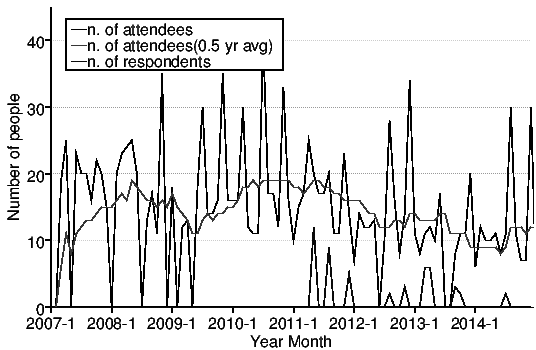
\includegraphics[width=.6\hsize]{image201412/memberanalysis/kansai_mono.png}
  \end{center}
  \caption{関西の参加人数推移(参加人数と6ヶ月移動平均、アンケート回答人数)}
  \label{fig:kansaipeoplechart}
\end{figure}

%\pagebreak

\begin{table}
  \begin{minipage}{.5\linewidth}
    \caption{関西Debian勉強会の参加人数とトピック(2007-2008)}
    \begin{center}
      \begin{tabular}{|l|c|p{10em}|}
        \hline
        開催年月   & 参加人数 & 内容 \\
        \hline
        2007年3月  & 19       & 開催にあたり \\
        2007年4月  & 25       & goodbye、youtube、プロジェクトトラッカー\\
        2007年6月  & 23       & 社会契約、テーマ、debian/rules、bugreport\\
        2007年7月  & 20前後   & OSC-Kansai \\
        2007年8月  & 20       & Inkscape、patch、dpatch\\
        2007年9月  & 16       & ライブラリ、翻訳、debtorrent\\
        2007年10月 & 22       & 日本語入力、SPAMフィルタ\\
        2007年11月 & 20前後   & KOF \\
        2007年12月 & 15       & 忘年会、iPod touch\\
        \hline
        \hline
        開催年月   & 参加人数 & 内容 \\
        \hline
        2008年2月  & 20       & PC Cluster, GIS, \TeX \\
        2008年3月  & 23       & bug report, developer corner, GPG \\
        2008年4月  & 24       & coLinux, Debian GNU/kFreeBSD, sid \\
        2008年5月  & 25       & ipv6, emacs, ustream.tv\\
        2008年6月  & 20       & pbuilder, hotplug, ssl\\
        2008年8月  & 13       & coLinux \\
        2008年9月  & 17       & debian mentors, ubiquity, DFSG\\
        2008年10月 & 11       & cdbs,cdn.debian.or.jp \\
        2008年11月 & 35       & KOF \\
        2008年12月 & ?        & TeX資料作成ハンズオン\\
        \hline
      \end{tabular}
    \end{center}
  \end{minipage}
  \pagebreak
  \begin{minipage}{.5\linewidth}
    \begin{center}
      \caption{関西Debian勉強会の参加人数とトピック(2009-2010)}
      \begin{tabular}{|l|c|p{10em}|}
        \hline
        開催年月   & 参加人数 & 内容 \\
        \hline
        2009年1月  & 18       & DMCK, LT \\
        2009年3月  & 12       & Git \\
        2009年4月  & 13       & Installing sid, Mancoosi, keysign \\
p        2009年6月  & 18       & Debian Live, bash\\
        2009年7月  & 30?      & OSC2009Kansai \\
        2009年8月  & 14       & DDTSS, lintian \\
        2009年9月  & 14       & reportbug, debian mentors\\
        2009年10月 & 16       & gdb, packaging \\
        2009年11月 & 35       & KOF2009 \\
        2009年12月 & 16       & GPS program, OpenStreetMap \\
        \hline
        \hline
        開催年月   & 参加人数 & 内容 \\
        \hline
        2010年1月  & 16       & Xen, 2010年企画 \\
        2010年2月  & 16       & レンタルサーバでの利用, GAE \\
        2010年3月  & 30?      & OSC2010Kobe \\
        2010年4月  & 12       & デスクトップ環境, 正規表現 \\
        2010年5月  & 11       & ubuntu, squeeze \\
        2010年6月  & 11       & debhelper7, cdbs, puppet \\
        2010年7月  & 40?      & OSC2010Kyoto \\
        2010年8月  & 17       & emdebian, kFreeBSD \\pp
        2010年9月  & 17       & タイルWM \\
        2010年10月 & 12       & initramfs, debian live \\
        2010年11月 & 33       & KOF2010 \\
        2010年12月 & 14       & Proxmox, annual review \\
        \hline
      \end{tabular}
    \end{center}
  \end{minipage}
\end{table}

\begin{table}
  \begin{minipage}{.5\linewidth}
    \caption{関西Debian勉強会の参加人数とトピック(2011-2012)}
    \begin{center}
      \begin{tabular}{|l|c|c|p{10em}|}
        \hline
        開催年月  & 参加 & 回答 & 内容 \\
        \hline
        2011年1月 &10    & 0    & BTS, kFreeBSD\\
        2011年2月 &15    & 0    & pbuilder, Squeezeリリースパーティ\\
        2011年3月 &17    & 0    & ライセンス, ドキュメント\\
        2011年4月 &25    & 0    & OSC Kansai@Kobe \\
        2011年5月 &20    &12    & vi, dpkg \\
        2011年6月 &17    & 0    & vcs-buildpackage\{svn, git\}, IPv6\\
        2011年7月 &17    & 0    & OSC Kansai@Kyoto \\
        2011年8月 &20    & 9    & パッケージ作成ハンズオン\\
        2011年9月 &11    & 0    & vcs-buildpackage\{bzr, git\}\\
        2011年10月&11    & 0    & Emacs, vim 拡張のDebianパッケージ, 翻訳\\
        2011年11月&23    & 0    & KOF 2011\\
        2011年12月&13    & 5    & NMプロセス, BTS\\
        \hline
        \hline
        開催年月  & 参加 & 回答 & 内容 \\
        \hline
        2012年1月 & 7    &0     & Debian温泉合宿 \\
        2012年2月 &14    &0     & autofs+pam\_chroot, t-code, Debian Policy \\
        2012年3月 &12    &0     & Konoha, t-code, Debian Policy \\
        2012年4月 &12    &0     & フリーソフトウェアと著作権, Konoha, Debian Policy \\
        2012年5月 &13    &0     & DebianとLDAP(頓挫), ITP入門, Debian Policy \\
        2012年6月 & -    &0     & 大統一Debian勉強会 \\
        2012年7月 &10    &0     & DebianとLDAP, Debian Policy \\
        2012年8月 &28    &2     & OSC Kansai@Kyoto \\
        2012年8月 &16    &0     & DebianとKerberos, News from EDOS \\
        2012年9月 & 8    &0     & clang, Debian Policy \\
        2012年10月&14    &3     & 翻訳環境構築, DSAの舞台裏\\
        2012年11月&34    &0     & KOF 2012\\
        2012年12月&12    &0     & Debian on Android, Debian Policy \\
        \hline
      \end{tabular}
    \end{center}
  \end{minipage}
  \pagebreak
  \begin{minipage}{.5\linewidth}
    \caption{関西Debian勉強会の参加人数とトピック(2013)}
    \begin{center}
      \begin{tabular}{|l|c|c|p{10em}|}
        \hline
        開催年月  & 参加 & 回答 & 内容 \\
        \hline
        2013年1月 & 8    &0     & Using Drupal on Debian, 月刊Debian Policy その8 \\
        2013年2月 &11    &6     & Debian Installerトラブルシューティング, Ruby In Wheezy \\
        2013年3月 &12    &6     & UbuntuとGNOME Shellと私, 管理者視点からのGNOMEの大規模な配置 \\
        2013年4月 &10    &0     & リリースノートを読んでみよう。, \\
                  &      &      & クラウド初心者がAWSにDebianをのっけて翻訳サービスの試行に挑戦してみた \\
        2013年5月 &17    &0     & DebianとUbuntuの違いを知ろう, Debianの歩き方 \\
        2013年6月 & -    &0     & 大統一Debian勉強会 \\
        2013年7月 &      &0     & OSC 2013 Kansai @ Kyoto, GPG キーサインパーティ\\
        2013年8月 & 8    &3     & puppetによる構成管理の実践 \\
        2013年9月 &11    &2     & Linuxとサウンドシステム, dgitでソースパッケージを触ってみる \\
        2013年10月&11    &0     & ALSAのユーザーランド解説, git-buildpackage入門again \\
        2013年11月&20    &0     & KOF 2013 \\
        2013年12月& 6    &0     & 2013年の振り返りと2014年の企画, 忘年会 \\
        \hline
      \end{tabular}
    \end{center}
  \end{minipage}
\end{table}

\begin{table}
    \caption{関西Debian勉強会の参加人数とトピック(2014)}
    \label{tab:count2014kansai}
    \begin{center}
%      \begin{tabular}{|l|c|c|p{10em}|}
      \begin{tabular}{|l|c|c|l|}
        \hline
        開催年月  & 参加人数 & 回答人数 & 内容 \\
        \hline
        2014年1月 &12        &0         & LT, もくもくの会 \\
        2014年2月 &10        &0         & もくもくの会 \\
        2014年3月 &10        &0         & Debian で楽しむ 3D プリンティング, もくもくの会 \\
        2014年4月 &11        &0         & 自宅サーバにkvmを導入してみよう, Notmuch Mail, もくもくの会 \\
        2014年5月 & 8        &0         & もくもくの会 \\
        2014年6月 &11        &2         & Debian での systemd とのつきあい方, Linuxのドライバメンテナになった体験記, \\
                  &          &          & キーサイン, もくもくの会 \\
        2014年8月 &30        &0         & OSC 2014 Kansai @ Kyoto \\
                  &11        &0         & もくもくの会 \\
        2014年9月 & 7        &0         & もくもくの会 \\
        2014年10月& 7        &0         & もくもくの会 \\
        2014年11月&30        &0         & KOF 2014 \\
                  & 4        &0         & インストーラテスト, もくもくの会 \\
        2014年12月& 9        &0         & 2014年の振り返りと2015年の企画, 忘年会 \\
        \hline
      \end{tabular}
    \end{center}
\end{table}

%201412tokyo
%DebianとFedoraでパッケージをリリースするまでの話
%https://github.com/kenhys/rabbit-slide-kenhys-tokyodebian-groonga-201412/blob/master/tokyodebian-groonga-201412.rab

%201501kansai
%Bug Squash Party
%DebianのBugの眺め方  佐々木洋平 資料無し

%201502kansai
%ライトニングトーク 資料無し

%201503kansai
%某所 VPS を先走って Jessie に上げてみた 佐々木洋平 資料無し

%201502tokyoosc
%Debian Update 岩松 http://tokyodebian.alioth.debian.org/pdf/debianmeetingresume201502-osc2015-presentation.pdf

%201505kansai
%Jessie落穂拾い かわだてつたろう 資料無し

\clearpage
%-------------------------------------------------------------------------------
\dancersection{Debian Trivia Quiz}{野島 貴英}
%-------------------------------------------------------------------------------

ところで、みなさん Debian 関連の話題においついていますか?Debian関連の話
題はメーリングリストをよんでいると追跡できます。ただよんでいるだけではは
りあいがないので、理解度のテストをします。特に一人だけでは意味がわからな
いところもあるかも知れません。みんなで一緒に読んでみましょう。

今回の出題範囲は\url{debian-devel-announce@lists.debian.org} や \url{debian-devel@lists.debian.org}に投稿された
内容とDebian Project Newsからです。

\begin{multicols}{2}
%; whizzy-master ../debianmeetingresume201311.tex
% $B0J>e$N@_Dj$r$7$F$$$k$?$a!"$3$N%U%!%$%k$G(B M-x whizzytex $B$9$k$H!"(Bwhizzytex$B$,MxMQ$G$-$^$9!#(B
%

\santaku
{2014/11$B7nCf=\$K$F(BDebconf15$B$N%9%]%s%5!<$H$J$C$?4k6H$O2?<R$"$k$G$7$g$&!)(B}
{3$B<R(B}
{9$B<R(B}
{11$B<R(B}
{C}
{$B%9%]%s%5!<4k6H0lMw!'(Bcredativ, sipgate, Matanel Foundation, Google,
Fairsight Security, Martin Alfke / Buero 2.0, Ubuntu, Mirantis, Logilab,
Netways,Hetzner$B!#$5$"!*F|K\4k6H$N3'MM$b@'Hs$40l=o$K!*(B}

\santaku
{2014/11/18$B$K?k$K%0%i%UI=<(5!G=IU$-EEBn$G(BDebian$B$rF0$+$7$?6/<T$,8=$l$?;v$,OCBj$K$J$C$F$$$^$7$?!#;H$o$l$?EEBn$N%a!<%+$O$I$l!)(B}
{Texus Instruments$B<R(B}
{CASIO$B<R(B}
{Hewllet Packard$B<R(B}
{A}
{$B>\$7$/$O!'(Bhttp://hackaday.com/2014/11/18/ running-debian-on-a-graphing-calculator/$B!#;H$o$l$?EEBn$N@=IJL>$O!'(BTI-NSpire CX$B$H$$$&%7%j!<%:$N5!<o$@$=$&$G$9!#(B}

\santaku
{Debian$B%W%m%8%'%/%H$K$F(Binit$B%7%9%F%`$N%"%W%j%1!<%7%g%s$N0MB8EY$K4X$9$k(BGeneral Resolution$B$NEjI<$,9T$o$l$^$7$?!#EjI<$N7k2L$O!)(B}
{$B%Q%C%1!<%8$OFCDj$N(Binit$B%7%9%F%`$N$_$K0MB8$7$F$O$J$i$J$$(B}
{$B%Q%C%1!<%8%a%s%F%J$,K>$a$P!"FCDj$N(Binit$B%7%9%F%`$K0MB8$7$F$b(BOK}
{General Resoultion$B$OITMW$@(B}
{C}
{Debian$B$G$b(Binit system$B$H%Q%C%1!<%8$H$ND4@0$,0z$-B3$-0l@87|L?9T$o$l$F$$$^$9!#(B}

\santaku
{Debian Med$B%a%?%Q%C%1!<%8$N%P!<%8%g%s$,(B1.99$B$X0l5$$K%8%c%s%W$9$kM=Dj$G$"$k$3$H$,%"%J%&%s%9$5$l$^$7$?!#$3$N;~=i$a$FEk:\$5$l$kM=Dj$N0eNE4X78<T8~$1%7%9%F%`$O2?!)(B}
{$B0dEA;R2r@O%7%9%F%`(B}
{$B302J<j=QMQ%m%\%C%H%7%9%F%`(B}
{$BIB1!>pJs%7%9%F%`(B(HIS)}
{C}
{Debian Med$B%A!<%`$N:#2s$N4hD%$j$OAG@2$i$7$/!"(BPHYLP$B$N%i%$%;%s%9$rD9G/$N8r>D$NKv!"(BDFSG$B=`5r$N$b$N$KJQ99$7$F$b$i$&$J$I!"0eNE4X78<T$i!&@8J*3X4X78<T$i$KMM!9$K%]%8%F%#%V$J1F6A$rM?$($F$$$^$9!#$3$N3hF0$O0eNEJ,Ln$N3X=Q7O$N>pJs%5%$%H(BBioMedCentral$B$K(B''Community-driven development for computational biology at Sprints, Hackathons and Codefests''$B$H$$$&$3$H$G<h$j>e$2$i$l$?$=$&$G$9!#(B}

\santaku
{2014/11/14$B$K(BDebian$B$N(BBTS$B$K!"(BDebian$B$N%Q%C%1!<%83+H/=i?4<T$X=$@5:n6H$,NI$$1i=,$H$J$k$h$&$J%P%0$K4X$9$k(Btag$B$,@_$1$i$l$^$7$?!#0J2<$N$I$l(B}
{newcomer}
{gift}
{easeofcake}
{A}
{$B:#$^$G%Q%C%1!<%83+H/=i?4<T8~$1$K3d$jEv$F$i$l$F$$$?(BBTS$B$N(Btag$B$O(Bgift$B$G$7$?$,!"(Bnewcomer$B$XJQ$o$k$=$&$G$9!#0JA0$N(Bgift$B$H$$$&(Btag$BL>$@$H$A$g$C$HH=$j$K$/$$$H$N$3$H$G!":#2sL>A0JQ99$H$J$C$?$h$&$G$9!#(B}

\santaku
{Mysql$B$K4X$9$k2>A[%Q%C%1!<%8$KDj5A$5$l$?(BMysqlDB$B8_49(BDB$B%=%U%H$H$7$F(BPXC$B$H$$$&$N$,$"$k$,!"$3$A$i$O2?$NN,!)(B}
{Protected eXchange Controler}
{Posgresql eXtra Controler}
{Percona XtraDB Cluster}
{C}
{Debian$B$K$F!"(BMysql$B7O$N(BDB$B$H$_$J$5$l$?$b$N$O!"#3$D$"$j!"(BMysqlDB,MariaDB,Percona XtraDB Cluster(PCX)$B$N#3$D$H$J$j$^$9!#(B}

\santaku
{2014/11/20$B$K$F!"(Bsystemd$BMQ$NDj5A%U%!%$%kFbIt$G;H$($k%;%-%e%j%F%#$rBgI}$K8~>e=PMh$k%*%W%7%g%s$N$&$A!"%[!<%`%G%#%l%/%H%j$NIT@5%"%/%;%9$rM^;_$9$k$N$O<!$N$I$l(B}
{ProtectHome}
{ProtectSystem}
{PrivateTmp}
{A}
{systemd$B$NDj5A%U%!%$%k$KMQ0U$5$l$F$$$k%;%-%e%j%F%#$K4X$9$k%*%W%7%g%s$r$&$^$/;H$$$3$J$9$HHs>o$K6/8G$J%7%9%F%`$K$9$k$3$H$,=PMh$k$=$&$G$9!#%N%&%O%&$H>R2p$O(Bhttp://0pointer.net/public/systemd-nluug-2014.pdf}















%; whizzy-master ../debianmeetingresume201311.tex
% $B0J>e$N@_Dj$r$7$F$$$k$?$a!"$3$N%U%!%$%k$G(B M-x whizzytex $B$9$k$H!"(Bwhizzytex$B$,MxMQ$G$-$^$9!#(B
%

\santaku
{12/29$B$K!"(BDebian$B$N%5!<%S%9$HO"7H$G$-$k(Bchromium$B8~$1$N3HD%5!G=$,%j%j!<%9$5$l$^$7$?!#2?$HO"7H$G$-$k$N$G$7$g$&$+!)(B}
{tracker.debian.org}
{sources.debian.net}
{www.debian.or.jp}
{B}
{zack$B$5$s$N(BDebconf14$B$N%W%l%<%s$r8+$F%$%s%9%Q%$%"$5$l$?$H$N$3$H$G!"(BRaphael Geissert$B$5$s$,:n$C$?(Bchromium$BMQ(B(chrome$B$G$bF0$/!K$N%*%s%i%$%s%=!<%9%3!<%I%(%G%#%?$r<B8=$9$k3HD%5!G=$G$9!#(BDebian$B%Q%C%1!<%8$N%=!<%9%3!<%I$rD>@\%*%s%i%$%s$G1\Mw$G$-$k(Bsources.debian.net$B>e$N%3!<%I$r$3$N3HD%5!G=$r;H$C$F%7!<%`%l%9$KJT=82DG=$K$J$j$^$9!#(Bzack$B$5$s$N<($7$??<9o$JLdBj!JBh(B117$B2sEl5~%(%j%"(BDebian$BJY6/2q;qNA;2>H!K$r2r7h$9$k0Y$N2h4|E*$J%"%$%G%"$N#1$D$G$9!*%^%B$9$P$i$7$$!*<+M3%=%U%H%&%'%"%i%V!"(BDebian$B%i%V$J?M$O!"AaB.!"(Bchromium$B$X(BNautilus$B$+$i$3$N3HD%5!G=$rEj$29~$s$G;n$9$Y$7!*(B}

\santaku
{2014/11/11$B$K(BRapha\"el Hertzog$B$5$s$K$h$jDs0F$5$l$?(BDEP14$B$NFbMF$O0J2<$N$I$l!)(B}
{git$B%Q%C%1!<%8%s%0%j%]%8%H%j$N;H$$J}$K$D$$$F(B}
{control$B%U%!%$%k$K(BDebian-Homepage$B%U%#!<%k%I$rF~$l$k7o(B}
{debian/upstream/metadata$B$rMQ0U$9$k7o(B}
{A}
{$B%Q%C%1!<%8%s%0%j%]%8%H%j$N%V%i%s%A$H%?%0$K%Y%s%@!<>pJs!JNc!'(Bdebian/*,ubuntu/*)$B$d$i%P!<%8%g%s>pJs$NF~$lJ}$J$I$r4^$`!"=t!9$N%k!<%k$NDs0F!#>\$7$/$O!"(Bhttp://dep.debian.net/deps/dep14/$B;2>H!#$J$*!"(BDebian-Homepage$B%U%#!<%k%I$N7o$O(BDEP13$B!#(Bdebian/upstream/metadata$B$N7o$O(BDEP12$B!#(B}

\santaku
{2015/1/8 Marvel$B<R$h$j(BDebian ARM$BMQ%Q%C%1!<%8%S%k%I%^%7%s$N4sIU$,$"$j$^$7$?!#$5$F2?Bf$NDs6!$,$"$C$?$G$7$g$&!)(B}
{7$BBf(B}
{8$BBf(B}
{10$BBf(B}
{B}
{Marvel$B<R$,Ds6!$7$?%5!<%P$O(B MV78460 SoC$B%Y!<%9$N%\!<%I(B8$B$D$rDs6!$H$N$3$H!#$J$*!"(BMV78460$B$O!"(BARM v7$B%3%"#44p$rEk:\$9$k(BMarvel$B<R3+H/$N(BSoC$B!#;29M!'(Bhttp://www.marvell.com/embedded-processors/armada-xp/}

\santaku
{2015/1/10$B$K(Bwheezy$B$,%"%C%W%G!<%H$5$l$^$7$?!#$5$F%P!<%8%g%s$O<!$N$I$l!#(B}
{7.6}
{7.7}
{7.8}
{C}
{wheezy$B$r$*;H$$$NJ}!9$OAaB.%"%C%W%0%l!<%I$7$^$7$g$&!#(B}

\santaku
{2015/1/1$B$K$"$kD9$5L$K~$N(BDebian keyring$B$N>C5n$,40N;$7$?$=$&$G$9!#$"$kD9$5$H$O(B?}
{2048}
{4096}
{8192}
{A}
{$B%"%J%&%s%9$H!">C$5$l$?3:Ev$N%-!<0lMw$O(Bdebian-devel-announce$B$N(B2015/1/1$B$N5-;v$K5-:\$,$"$j$^$9!#(Bhttps://lists.debian.org/debian-devel-announce/2015/01/msg00000.html}

\santaku
{2014/12/6$B$K(Bcdn.debian.net$B$N%l%3!<%I$N<($9@h$r!"$H$"$k(BFQDN$B$N(BCNAME$B$H$7$?$$;]$NLd$$9g$o$;$,(Bdebian-devel ML$B$K$"$j$^$7$?!#$I$3$K8~$1$k!)(B}
{ftp.debian.or.jp}
{ftp.jp.debian.org}
{http.debian.net}
{C}
{cdn.debian.net$B$rDs6!$7$F$$$k(BAraki$B$5$s$+$i$NLd$$9g$o$;!#(Bsqueeze$B0J>e$GEk:\$5$l$F$$$k(Bapt ver 0.7.21$B$G$O(Bhttp$B$N(Bredirect$B$KBP1~$7$F$$$k$N$G!"MxMQ<T$K:G$b6a$$%Q%C%1!<%8%@%&%s%m!<%I@h$r65$($F$/$l$k5!9=$r(Bhttp.debian.net$B$K0lK\2=$7$?$$$H$N$3$H!#FC$KH?BP$9$k?M$O5o$J$$LOMM$G$9!#(B}

\santaku
{2015/1/9$B$K(Bdebian-devel ML$B$K$F!"0lIt%Q%C%1!<%8$N(Bdescription$B$,D9$9$.$k7o$K$D$$$F$N5DO@$,$"$j$^$7$?!#:G$bD9$$(Bdescription$B$N9T$r;}$D%Q%C%1!<%8$O<!$N$I$l!)(B}
{firmware-linux-nonfree}
{texlive-latex-extra}
{irssi-scripts}
{B}
{2015/1/9$B8=:_!"(Bunstable/main$B$G$O!":G$bD9$$9T?t$N=g$G$$$/$H!"(B1$B0L(B texlive-latex-extra($B<B$K(B1935$B9T(B!!)$B!"(B2$B0L(B texlive-fonts-extra(437$B9T(B)$B!"(B3$B0L(B irssi-scripts(350$B9T(B)$B!#(Bunstable/non-free$B$G$O!"(B1$B0L(B firmware-linux-nonfree(251$B9T(B)$B$G$9!#(B}



%; whizzy-master ../debianmeetingresume201311.tex
% $B0J>e$N@_Dj$r$7$F$$$k$?$a!"$3$N%U%!%$%k$G(B M-x whizzytex $B$9$k$H!"(Bwhizzytex$B$,MxMQ$G$-$^$9!#(B
%

\santaku
{2015/2/6$B$K!"$H$"$k9q$K(Bsecurity mirror$B$,?7@_$5$l$?$3$H$,%"%J%&%s%9$5$l$^$7$?!#$I$3$N9q!)(B}
{$BF|K\(B}
{$B%"%a%j%+(B}
{$B%8%c%^%$%+(B}
{A}
{Debian$B$N(Bsecurity mirror$B$r?7@_$7$F$$$?$@$$$?$N$O!"(BSAKURA Internet$B$5$s(B(http://www.sakura.ad.jp/)$B$H$J$j$^$9!#$3$A$i$"$j$,$H$&$4$6$$$^$9!*(BOSC 2015 Tokyo/Spring(http://www.ospn.jp/osc2015-spring/)$B$X9T$+$l$kJ}$O!"(BSAKURA Internet$B$5$s$N%V!<%9$K$F$h$m$7$/$*EA$($/$@$5$$$^$;!*$^$?!"$3$A$i$N?7@_$K?TNO$5$l$?!"$d$^$M$5$s$H(BDebian JP Project$B$N4X78<T$N3'MM!"$*Hh$l$5$^$G$7$?!*(B}

\santaku
{2015/1/26$B$K!"(BDebian Installer$B$N%j%j!<%9$N%"%J%&%s%9$,$5$l$^$7$?!#$3$A$i$N%P!<%8%g%s$O$$$/$D!)(B}
{Jessie RC 1}
{Jessie RC 2}
{Jessie RC 3}
{A}
{Debian Installer$B$N%j%j!<%9$NOC$G!"(BJessie$BK\BN$N%j%j!<%9$NOC$G$OL5$$$G$9!#$G!":#2s(B1/26$B$K(BRC1$B$,%j%j!<%9$5$l$?$3$H$,%"%J%&%s%9$5$l$^$7$?!#%P%0=P$7!"FC$K(BUEFI$B4D6-$r$*$b$A$NJ}!"F0:n%F%9%H$7$F%P%0=P$7$H(BBTS$B$X$N%l%]!<%H$h$m$7$/$*$M$,$$$7$^$9!<!#(B}

\santaku
{$B2a5n$K=t!9$NM}M3$K$h$j(Btesting$B$+$i(BRemove$B$5$l$F$7$^$C$?(BJessie$B8~$1$N%Q%C%1!<%8$K$D$$$F!":FEYI|3h$G$-$k:G8e$N%A%c%s%9$NDy@Z$jF|$O$$$D$G$7$g$&!)(B}
{2/5$BCf(B}
{2/14$BCf(B}
{2$B7nKvCf(B}
{A}
{2/5 23:59:59 UTC$B$^$G$@$=$&$G$9!#$b$&=*$o$C$A$c$$$^$7$?$M!#3'MM$N%Q%C%1!<%8$OL5;v$G$7$?$G$7$g$&$+!)(B}

\santaku
{2015/2/13$B$K$F(BGSoC 2015$B$N(BDebian$B$K4X$9$k%W%m%8%'%/%HJg=8$H(BGSoC$B$N%a%s%?!<Jg=8$,9T$o$l$^$7$?!#(B2/15$B8=:_4s$;$i$l$F$$$J$$%W%m%8%'%/%H$O!)(B}
{Apport of Debian}
{Coinstallable PHP Versions}
{Debian Gnu/Hurd enhancements}
{C}
{$B>\$7$/$O!"(Bhttps://wiki.debian.org/SummerOfCode2015/Projects$B!#(BApport$B$O!"%W%m%0%i%`$,%/%i%C%7%e$7$?$H$-$K3d$j9~$_!"%G%P%C%0>pJs$d4D6-$N>pJs$r(BBTS$B$XAw$k%7%9%F%`!#(BCoinstallable PHP Version$B$O(BDebian$B$K$F!"(Bphp 5.X$B$N3F%P!<%8%g%s$4$H$N(BPHP$B%Q%C%1!<%8(B/PHP$B4D6-$rF15o$7$FF3F~$G$-$k$h$&$K$9$k%W%m%8%'%/%H!#(B}

\santaku
{2015/2/13$B$K(BReproducible Builds$B$NJs9p$,$"$j$^$7$?!#8=:_(Bmain$B%Q%C%1!<%8$N2?(B\%$B$,40N;$7$F$$$k$G$7$g$&!)(B}
{62\%}
{83\%}
{100\%}
{B}
{Reproducible Builds$B$H$O!"8=:_$*;H$$$N(BDebian$B$N3F%P%$%J%j%Q%C%1!<%8$,!"K\Ev$K8=:_$N%=!<%9%Q%C%1!<%8$+$i@8@.$5$l$?$b$N$G!"0-0U$N$"$k%P%$%J%j$,:.$8$C$F$$$J$$$+$rD4$Y$k;n$_!#4JC1$K8@$&$H!"%=%U%H@=B$<TB&$N@=IJK\BN$N%&%#%k%946@w%A%'%C%/$_$?$$$J$b$N!#(BDebian$B$NB>$K$b!"(BFedora/OpenSUSE/NixOS$B$G$b9T$o$l$F$$$k!#>\$7$/$O(B https://wiki.debian.org/ReproducibleBuilds$B!#$^$?!"K\%W%m%8%'%/%H$N$K$D$$$F$N%W%l%<%s$O!'(Bhttp://reproducible.alioth.debian.org/presentations/2014-02-01-FOSDEM14.pdf}

%; whizzy-master ../debianmeetingresume201311.tex
% $B0J>e$N@_Dj$r$7$F$$$k$?$a!"$3$N%U%!%$%k$G(B M-x whizzytex $B$9$k$H!"(Bwhizzytex$B$,MxMQ$G$-$^$9!#(B
%

\santaku
{2015/3/3$B$K(BDebConf15$B$N%"%J%&%s%9$,9T$o$l$^$7$?!#%9%]%s%5!<%I$J;22C$NEPO?4|8B$O2?;~$^$G$G$7$g$&!)(B}
{2015/3/7}
{2015/3/15}
{2015/3/29}
{C}
{$B=IGqBe$H?);v$,(BDebConf$B3+:EB&;}$A$H$J$k%9%]%s%5!<%I$J;22CEPO?$N!:@Z$O(B3/29$B$G$9!*!:@Z$N;~9o$O(BUTC$B$J$N$+!"%I%$%D$N%m!<%+%k%?%$%`$+!":Y$+$$;v$,$o$+$i$J$$$N$G!";22C$r8!F$$5$l$F$$$kJ}$O!:@Z$KBP$7$F==J,$KF|Dx$NM>M5$r$b$C$FEPO?$5$l$k;v$r$*$9$9$a$7$^$9!#(BDebConf15$B$O!"%I%$%D(B $B%O%$%G%k%P!<%0$G(B2015/8/15-22$B$N3+:E$G$9!#(BDebCamp$B$O!"(B8/9-8/14$B$H$J$j$^$9!#(B}

\santaku
{2015/3/4$B$K(BDPL$B$N:#G/$NA*=P$K$D$$$F%"%J%&%s%9$,$"$j$^$7$?!#(BDPL$B$NN)8uJd!:@Z$O2?;~!)(B}
{2015/3/4}
{2015/3/9}
{2015/4/1}
{B}
{$BKhG/91Nc$N(BDPL$BA*5s$G$9!#(BDPL$B$NN)8uJd!:@Z$O(B3/9$B$G!"A*5s$O(B4/1$B$+$i9T$o$l$^$9!#:#G/$OC/$,N)8uJd$9$k$N$G$7$g$&$+!)$^$?!"F1;~$K!"(BDebian JP Project$B$K$D$$$F$b!"(B2015$BG/$N2qD9$NN)8uJd<TJg=8$,9T$o$l$F$$$^$9!#(B}

\santaku
{2015/3/1$B$K$F!"(BAraki$B$5$s$h$j!"(B2007$BG/$+$i2TF/$7$F$$$?(Bcdn.debian.net$B$,$=$NLr3d$r=*$(!"$"$k(BFQDN$B$r;X$9$@$1$K$J$k$H$$$&$3$H$,%"%J%&%s%9$5$l$^$7$?!#$3$N(BFQDN$B$O0J2<$N$I$l!)(B}
{ftp.debian.org}
{http.debian.net}
{sources.debain.net}
{B}
{cdn.debian.net$B$O!"(Bapt$B$K$h$k(BDebian$B%Q%C%1!<%8$N<hF@@h$K$D$$$F!"(BDNS$B%/%(%j$NH/9T$5$l$?>l=j$K4p$E$$$F!"%f!<%6$K:G$b6a$$%Q%C%1!<%8%j%]%8%H%j$N%5!<%P$N(BIP$B%"%I%l%9$r(BDNS$B$N%l%3!<%I$GJV5Q$9$k;EAH$_$G$9!#(BAraki$B$5$s$K$h$C$F@_7W!"9=C[!"1?MQ$5$l$F$*$j$^$7$?!#(B2010$BG/$K(Bapt$B$,(BHTTP $B%j%@%$%l%/%H$r%5%]!<%H$G$-$k$h$&$K$J$C$?$?$a!"(Bcdn.debian.net$B$N5!G=$r(BHTTP$B$N%j%@%$%l%/%H5!G=$G<B8=$9$k(Bhttp.debian.net$B$,1?MQ$5$l$F$-$^$7$?!#:#2s!"?k$K!"(Bcdn.debian.net$B$r0zB`$5$;$k%"%J%&%s%9$,9T$o$l$?$H$$$&>u67$G$9!#$b$7!"(Bsource.list$B$K(Bcdn.debian.net$B$N(BFQDN$B$r;XDj$7$F$$$k>l9g$O!"(Bhttp.debian.net$B$KJQ$($^$7$g$&!#(B}



%; whizzy-master ../debianmeetingresume201311.tex
% 以上の設定をしているため、このファイルで M-x whizzytex すると、whizzytexが利用できます。
%

\santaku
{2015/2/17にて、DPLのLucas Nussbaumにより立て直しの協力募集が行われたチームは?}
{DSA team}
{partners team}
{東京エリアDebian勉強会team}
{B}
{Debian Projectには、Debian パートナーズプログラム(https://www.debian.org/partners/)という制度があります。こちらを統括しているチームとしてpartners teamがあるのですが、昨今、こちらの構成員の時間が取れない状態らしく、対応が滞っているという状況のようです。なお、DSAはThe Debian System Administratorsというチームのことでバリバリ活動されてます。東京エリアDebian勉強会teamは当勉強会幹事の頭の中の妄想上のチームですが、頑張ってるぜ!}

\santaku
{2015/2/23に、Debianがクレジットに載せられた映画があることがindenti.caのzakの投稿で判りました。何と言う名前の映画?}
{ミレニアム ドラゴン・タトゥーの女}
{Toy Story}
{Citizenfour}
{C}
{Citizenfourというエドワード・スノーデンを題材にしたドキュメンタリー映画のクレジットのSpecial ThanksとしてDebianが入りました。imdbにもcompanyとして登録されました。Citizenfourは2015年アカデミー賞のうち長編ドキュメンタリー賞を受賞しました(http://www.imdb.com/company/co0504449/, http://www.huffingtonpost.jp/tatsuhei-morozumi/citizenfour\_b\_6741756.html)ギャガ株式会社配給で将来日本でも公開されるとのことですので、将来クレジットを確認すると良いかもしれません}

\santaku
{2015/3/31にJessieのリリース目標の日がアナウンスされました。いつでしょう?}
{4/1}
{4/18}
{4/25}
{C}
{遂に4/25がJessieのリリース目標の日取りとなりました。ただ、最悪のケースとして、Jessieにリリースに支障があるような非常に重大な問題が見つかり修正が間に合わない場合は、ずれる可能性があるとは記載されています。現在uddを参照すると、キーパッケージだけでも47個ぐらいRCバグが残ったままのようですので、Fix! Fix! なお、4/25に東京でリリースパーティーが企画されています。詳細はconnpassのDebian JPグループを見て下さいませ。}

\santaku
{2015/4/16のlucas最後のbit from DPLが流れました。こちらに記載されていたDebianからパッケージをリリースできるようにするための法的対策を検討中のソフトウェアは以下のどれ?}
{libdvdcss}
{OTR software}
{Unreal Engine4}
{A}
{なんと、libdvdcssと、ZFSが検討中らしい。もちろん、ダメになる可能性は十分にあるので、状況を静観したいと思います。libdvdcssはそのコード本体がクラッキング行為の塊なので、万一debianに入った場合、日本でdebianをミラーしても大丈夫かどうかは今後の議論ですね}

\santaku
{Debianにて開発者の属性の不均衡を正す事を目的として活動する公式チームがDebian Projectに新設したと4/16にlucasによりアナウンスがありました。なんという名前のチーム?}
{Debian Release team}
{Debian Outreach team}
{Technical Comittie}
{B}
{現在、是正すべき属性のターゲットとしては性別分布を目標としているようです。現在、Debian公式開発者の性別の割合は男性に大きく偏ってしまっています。Debianは多様性を重視するプロジェクトです。将来、性別の不均衡が是正されると良いですね。}

\santaku
{2015/4/15に選出された新DPLは誰?}
{Mehdi Dogguy}
{Gergely Nagy}
{Neil McGovern}
{C}
{Neil McGovernさんはDebian ProjectでRelease Teamで活動されるなど多数の貢献をされている方です(所信表明は:https://www.debian.org/vote/2014/platforms/neilm )。ちなみに、2015のDebian JP Project会長は岩松さんが選出されました。おめでとうございます。}







%; whizzy-master ../debianmeetingresume201311.tex
% 以上の設定をしているため、このファイルで M-x whizzytex すると、whizzytexが利用できます。
%

\santaku
{Jessieが無事リリースされました。いつだったでしょうか?}
{2015/4/11}
{2015/4/18}
{2015/4/25}
{C}
{無事4/25にJessie(Debian 8)がリリースされました。Linux kernelは3.16.7、GNU Compiler Collection 4.9.2、GNOME 3.14、Apache 2.4.10、PHP 5.6.7などのバージョンのものが搭載されました。搭載されているパッケージ数は全部で43,000パッケージ以上もあります。}

\santaku
{Jessieで初めて追加されたものではないものが混ざっています。どれ?}
{Debian Games Blend}
{OpenJDK}
{androidsdk-tools}
{B}
{Jessieでの変更点はリリースノート(https://www.debian.org/releases/ jessie/amd64/release-notes/index.ja.html)にあります。Debian Gamesチームよりゲームの詰め合わせのDebian Blendが追加されたり、androidの開発ツールの一部も追加されたりしています。}

\santaku
{Debian GNU/Hurd 2015も2015/4/30にリリースされました。心臓部のGNU Machのバージョンはいくつ?}
{1.6}
{1.5}
{1.4}
{B}
{2015/4/10〜2015/4/15周辺でGNU/Hurd(upstream側)のアップデートが行われ、GNU Hurdはversion 0.6に、GNU Machは1.5になりました。未だにKVM/QEMUなどの仮想環境での動作が推奨の32bitシステムですが、多くのOSがクラウド環境で動作している世の中ですので、ホビー用途の利用でそろそろ注目されても良いかも?と思う次第です。}

\santaku
{2015年のGSoCに採択された、Debian MIPS portsについての開発内容は次のどれ?}
{多数のビルド出来ないパッケージを、ちゃんとビルドできるようにする。}
{新しいMIPS CPUへの対応}
{新しいMIPS CPU搭載製品への対応}
{A}
{Debian MIPS portsの多数のパッケージは再ビルドが出来ない、インストールに失敗するものが多数ある状況です。こちらを再ビルドできるように修正し、インストール出来るようにする事が採択されました。GSoCに限らず、いつでも本件の協力者募集中ですので、MIPS portsに興味ある方はパッケージの修正に是非ご協力くださいませー。}

\santaku
{遂にhttp.debian.netがdebian.orgのインフラに移動となりました。新しいURLはどれ?}
{http://http.debian.org/debian}
{http://httpredir.debian.org/debian}
{http://www.debian.org/}
{B}
{http.debian.netはHTTPのRedirectを活用し、ユーザに最も適切な場所にある、パッケージのミラー先を教えてくれるサービスです。遂に、実験的サービスの扱いであるdebian.netからDebian公式サービスであるdebian.orgへ移動となりました。http.debian.netをsource.listに設定している人は、httpredir.debian.orgへ修正をおねがいします。また、不具合は"mirrors" pseudo-packageでBTSするようです。参照:http://bugs.debian.org/mirrors }

\santaku
{debianへのlibdvdcss/ZFSパッケージ搭載の件について、2015/5のBit From DPLで報告された状況は以下のどれ?}
{DPLがいろいろ議論して回っている状況}
{搭載日確定した}
{搭載を諦めた}
{A}
{2015/5/19現在、FTPMasters, SFLC, FSFと議論中とのこと。さらに近々Linux Foundationとも議論予定。現在、当初想定したよりも、実現に関する状況が複雑とのことで、本件いつ決着するか見えなくなったとの事です。}


\end{multicols}

% 索引
\printindex

% 問題と回答が同じみひらきにならないようにする
%\cleartoevenpage
%-------------------------------------------------------------------------------
\dancersection{Debian Trivia Quiz 問題回答}{野島 貴英}
%-------------------------------------------------------------------------------
\\
{\small
 Debian Trivia Quiz の問題回答です。 あなたは何問わかりましたか? \\
 %回答はdebianmeetingresume2015-natsu.jqzというファイルに生成されるので、
 %それを手動でコピペして使う。
 % ここからコピペ
 % FIXME 問題が全部はいったらコピペすること
1. C スポンサー企業一覧:credativ, sipgate, Matanel Foundation, Google, Farsight Security, Martin Alfke / Buero 2.0, Ubuntu, Mirantis, Logilab, Netways,Hetzner。さあ!日本企業の皆様も是非ご一緒に!\\
2. A 詳しくは:http://hackaday.com/2014/11/18/ running-debian-on-a-graphing-calculator/。使われた電卓の製品名は:TI-NSpire CXというシリーズの機種だそうです。\\
3. C Debianでもinit systemとパッケージとの調整が引き続き一生懸命行われています。\\
4. C Debian Medチームの今回の頑張りは素晴らしく、PHYLPのライセンスを長年の交渉の末、DFSG準拠のものに変更してもらうなど、医療関係者ら・生物学関係者らに様々にポジティブな影響を与えています。この活動は医療分野の学術系の情報サイトBioMedCentralに''Community-driven development for computational biology at Sprints, Hackathons and Codefests''ということで取り上げられたそうです。\\
5. A 今までパッケージ開発初心者向けに割り当てられていたBTSのtagはgiftでしたが、newcomerへ変わるそうです。以前のgiftというtag名だとちょっと判りにくいとのことで、今回名前変更となったようです。\\
6. C Debianにて、Mysql系のDBとみなされたものは、3つあり、MysqlDB,MariaDB,Percona XtraDB Cluster(PCX)の3つとなります。\\
7. A systemdの定義ファイルに用意されているセキュリティに関するオプションをうまく使いこなすと非常に強固なシステムにすることが出来るそうです。ノウハウと紹介はhttp://0pointer.net/public/systemd-nluug-2014.pdf\\
8. B zackさんのDebconf14のプレゼンを見てインスパイアされたとのことで、Raphael Geissertさんが作ったchromium用(chromeでも動く)のオンラインソースコードエディタを実現する拡張機能です。Debianパッケージのソースコードを直接オンラインで閲覧できるsources.debian.net上のコードをこの拡張機能を使ってシームレスに編集可能になります。zackさんの示した深刻な問題(第117回東京エリアDebian勉強会資料参照)を解決する為の画期的なアイデアの1つです!マヂすばらしい!自由ソフトウェアラブ、Debianラブな人は、早速、chromiumへNautilusからこの拡張機能を投げ込んで試すべし!\\
9. A パッケージングリポジトリのブランチとタグにベンダー情報(例:debian/*,ubuntu/*)やらバージョン情報の入れ方などを含む、諸々のルールの提案。詳しくは、http://dep.debian.net/deps/dep14/参照。なお、Debian-Homepageフィールドの件はDEP13。debian/upstream/metadataの件はDEP12。\\
10. B Marvel社が提供したサーバは MV78460 SoCベースのボード8つを提供とのこと。なお、MV78460は、ARM v7コア4基を搭載するMarvel社開発のSoC。参考:http://www.marvell.com/embedded-processors/armada-xp/\\
11. C wheezyをお使いの方々は早速アップグレードしましょう。\\
12. A アナウンスと、消された該当のキー一覧はdebian-devel-announceの2015/1/1の記事に記載があります。https://lists.debian.org/debian-devel-announce/2015/01/msg00000.html\\
13. C cdn.debian.netを提供しているArakiさんからの問い合わせ。squeeze以上で搭載されているapt ver 0.7.21ではhttpのredirectに対応しているので、利用者に最も近いパッケージダウンロード先を教えてくれる機構をhttp.debian.netに一本化したいとのこと。特に反対する人は居ない模様です。\\
14. B 2015/1/9現在、unstable/mainでは、最も長い行数の順でいくと、1位 texlive-latex-extra(実に1935行!!)、2位 texlive-fonts-extra(437行)、3位 irssi-scripts(350行)。unstable/non-freeでは、1位 firmware-linux-nonfree(251行)です。\\
15. A Debianのsecurity mirrorを新設していただいたのは、SAKURA Internetさん(http://www.sakura.ad.jp/)となります。こちらありがとうございます!OSC 2015 Tokyo/Spring(http://www.ospn.jp/osc2015-spring/)へ行かれる方は、SAKURA Internetさんのブースにてよろしくお伝えくださいませ!また、こちらの新設に尽力された、やまねさんとDebian JP Projectの関係者の皆様、お疲れさまでした!\\
16. A Debian Installerのリリースの話で、Jessie本体のリリースの話では無いです。で、今回1/26にRC1がリリースされたことがアナウンスされました。バグ出し、特にUEFI環境をおもちの方、動作テストしてバグ出しとBTSへのレポートよろしくおねがいしますー。\\
17. A 2/5 23:59:59 UTCまでだそうです。もう終わっちゃいましたね。皆様のパッケージは無事でしたでしょうか?\\
18. C 詳しくは、https://wiki.debian.org/SummerOfCode2015/Projects。Apportは、プログラムがクラッシュしたときに割り込み、デバッグ情報や環境の情報をBTSへ送るシステム。Coinstallable PHP VersionはDebianにて、php 5.Xの各バージョンごとのPHPパッケージ/PHP環境を同居して導入できるようにするプロジェクト。\\
19. B Reproducible Buildsとは、現在お使いのDebianの各バイナリパッケージが、本当に現在のソースパッケージから生成されたもので、悪意のあるバイナリが混じっていないかを調べる試み。簡単に言うと、ソフト製造者側の製品本体のウィルス感染チェックみたいなもの。Debianの他にも、Fedora/OpenSUSE/NixOSでも行われている。詳しくは https://wiki.debian.org/ReproducibleBuilds。また、本プロジェクトのについてのプレゼンは:http://reproducible.alioth.debian.org/presentations/2014-02-01-FOSDEM14.pdf\\
20. C 宿泊代と食事がDebConf開催側持ちとなるスポンサードな参加登録の〆切は3/29です!〆切の時刻はUTCなのか、ドイツのローカルタイムか、細かい事がわからないので、参加を検討されている方は〆切に対して十分に日程の余裕をもって登録される事をおすすめします。DebConf15は、ドイツ ハイデルバーグで2015/8/15-22の開催です。DebCampは、8/9-8/14となります。\\
21. B 毎年恒例のDPL選挙です。DPLの立候補〆切は3/9で、選挙は4/1から行われます。今年は誰が立候補するのでしょうか?また、同時に、Debian JP Projectについても、2015年の会長の立候補者募集が行われています。\\
22. B cdn.debian.netは、aptによるDebianパッケージの取得先について、DNSクエリの発行された場所に基づいて、ユーザに最も近いパッケージリポジトリのサーバのIPアドレスをDNSのレコードで返却する仕組みです。Arakiさんによって2007年頃にて設計、構築、運用されておりました。2010年にaptがHTTP リダイレクトをサポートできるようになったため、cdn.debian.netの機能をHTTPのリダイレクト機能で実現するhttp.debian.netが稼働を開始しました。今回、遂に、cdn.debian.netを引退させるアナウンスが行われたという状況です。もし、source.listにcdn.debian.netのFQDNを指定している場合は、http.debian.netに変えましょう。\\
23. B Debian Projectには、Debian パートナーズプログラム(https://www.debian.org/partners/)という制度があります。こちらを統括しているチームとしてpartners teamがあるのですが、昨今、こちらの構成員の時間が取れない状態らしく、対応が滞っているという状況のようです。なお、DSAはThe Debian System Administratorsというチームのことでバリバリ活動されてます。東京エリアDebian勉強会teamは当勉強会幹事の頭の中の妄想上のチームですが、頑張ってるぜ!\\
24. C Citizenfourというエドワード・スノーデンを題材にしたドキュメンタリー映画のクレジットのSpecial ThanksとしてDebianが入りました。imdbにもcompanyとして登録されました。Citizenfourは2015年アカデミー賞のうち長編ドキュメンタリー賞を受賞しました(http://www.imdb.com/company/co0504449/, http://www.huffingtonpost.jp/tatsuhei-morozumi/citizenfour\_b\_6741756.html)ギャガ株式会社配給で将来日本でも公開されるとのことですので、将来クレジットを確認すると良いかもしれません\\
25. C 遂に4/25がJessieのリリース目標の日取りとなりました。ただ、最悪のケースとして、Jessieにリリースに支障があるような非常に重大な問題が見つかり修正が間に合わない場合は、ずれる可能性があるとは記載されています。現在uddを参照すると、キーパッケージだけでも47個ぐらいRCバグが残ったままのようですので、Fix! Fix! なお、4/25に東京でリリースパーティーが企画されています。詳細はconnpassのDebian JPグループを見て下さいませ。\\
26. A なんと、libdvdcssと、ZFSが検討中らしい。もちろん、ダメになる可能性は十分にあるので、状況を静観したいと思います。libdvdcssはそのコード本体がクラッキング行為の塊なので、万一Debianに入った場合、日本でDebianをミラーしても大丈夫かどうかは今後の議論ですね\\
27. B 現在、是正すべき属性のターゲットとしては性別分布を目標としているようです。現在、Debian公式開発者の性別の割合は男性に大きく偏ってしまっています。Debianは多様性を重視するプロジェクトです。将来、性別の不均衡が是正されると良いですね。\\
28. C Neil McGovernさんはDebian ProjectでRelease Teamで活動されるなど多数の貢献をされている方です(所信表明は:https://www.debian.org/vote/2014/platforms/neilm )。ちなみに、2015のDebian JP Project会長は岩松さんが選出されました。おめでとうございます。\\
29. C 無事4/25にJessie(Debian 8)がリリースされました。Linux kernelは3.16.7、GNU Compiler Collection 4.9.2、GNOME 3.14、Apache 2.4.10、PHP 5.6.7などのバージョンのものが搭載されました。搭載されているパッケージ数は全部で43,000パッケージ以上もあります。\\
30. B Jessieでの変更点はリリースノート(https://www.debian.org/releases/ jessie/amd64/release-notes/index.ja.html)にあります。Debian Gamesチームよりゲームの詰め合わせのDebian Blendが追加されたり、androidの開発ツールの一部も追加されたりしています。\\
31. B 2015/4/10〜2015/4/15周辺でGNU/Hurd(upstream側)のアップデートが行われ、GNU Hurdはversion 0.6に、GNU Machは1.5になりました。未だにKVM/QEMUなどの仮想環境での動作が推奨の32bitシステムですが、多くのOSがクラウド環境で動作している世の中ですので、ホビー用途の利用でそろそろ注目されても良いかも?と思う次第です。\\
32. A Debian MIPS portsの多数のパッケージは再ビルドが出来ない、インストールに失敗するものが多数ある状況です。こちらを再ビルドできるように修正し、インストール出来るようにする事が採択されました。GSoCに限らず、いつでも本件の協力者募集中ですので、MIPS portsに興味ある方はパッケージの修正に是非ご協力くださいませー。\\
33. B http.debian.netはHTTPのRedirectを活用し、ユーザに最も適切な場所にある、パッケージのミラー先を教えてくれるサービスです。遂に、実験的サービスの扱いであるdebian.netからDebian公式サービスであるdebian.orgへ移動となりました。http.debian.netをsource.listに設定している人は、httpredir.debian.orgへ修正をおねがいします。また、不具合は"mirrors" pseudo-packageでBTSするようです。参照:http://bugs.debian.org/mirrors \\
34. A 2015/5/19現在、FTPMasters, SFLC, FSFと議論中とのこと。さらに近々Linux Foundationとも議論予定。現在、当初想定したよりも、実現に関する状況が複雑とのことで、本件いつ決着するか見えなくなったとの事です。\\

\pagestyle{empty}
\cleartoevenpage

\newpage
{
\large
\begin{itembox}{\bf 『あんどきゅめんてっど でびあん』について}
% FIXME: 回数を修正すること。
本書は、東京および関西周辺で毎月行なわれている『東京エリア Debian 勉強会』(第121回から第126回)および
『関西 Debian 勉強会』(第92回から第98回)で使用された資料・小ネタ・必殺技などを一冊にまとめたものです。
関西Debian勉強会資料の以下は収録無し。第93回はDebian Bug Squashing Party、第94回はライトニングトーク、
第95回は資料無し、第96回はDebian8 "Jessie" リリースパーティ。
内容は無保証、つっこみなどがあれば勉強会にて。
\end{itembox}
}

\vspace*{13cm}
{\color{dancerlightblue}\rule{\hsize}{1mm}}
\vspace{2mm}

\includegraphics[width=2cm]{image200502/openlogo-nd.eps}
\noindent \Large \bf あんどきゅめんてっど でびあん 2015年夏号\\
\noindent \normalfont 2015年8月16日 \hspace{5mm}  初版第1刷発行\\
\noindent \normalfont 東京エリア Debian 勉強会/関西エリア Debian 勉強会 (編集・印刷・発行)\\
{\color{dancerdarkblue}\rule{\hsize}{1mm}}

\end{document}
